% !TEX program = xelatex
% Modelo reduzido TEECII, Manual MSGQ-21.01 REV.16.

\documentclass[
    12pt,                % Tamanho da fonte base (corpo do texto)
    fleqn,               % Equações alinhadas à esquerda, com numeração à direita
    oneside,            % Impressão apenas em recto (frente das páginas)
    a4paper,            % Tamanho do papel: A4 (21.00 cm × 29.70 cm)
    chapter=TITLE,        % Títulos de capítulos convertidos em MAIÚSCULAS
    section=TITLE,        % Títulos de seções convertidos em MAIÚSCULAS  
    sumario=tradicional,% Estilo do sumário (tradicional = indentado)
    english,            % Idioma adicional para hifenização de termos técnicos
    brazil                % Idioma principal do documento (último da lista)
]{abntex2}

\usepackage{iftex}
\ifPDFTeX
    \usepackage[T1]{fontenc}
    \usepackage[utf8]{inputenc}
    \usepackage{helvet}
\else
    \usepackage{fontspec}
    \IfFileExists{fonts/arial.ttf}{
        \setmainfont{Arial}[
            Path=fonts/,
            Extension=.ttf,
            UprightFont=arial,
            BoldFont=arialbd,
            ItalicFont=ariali,
            BoldItalicFont=arialbi
        ]
        \setsansfont{Arial}[
            Path=fonts/,
            Extension=.ttf,
            UprightFont=arial,
            BoldFont=arialbd,
            ItalicFont=ariali,
            BoldItalicFont=arialbi
        ]
    }{
        \IfFileExists{fonts/Arial.ttf}{
            \setmainfont{Arial}[
                Path=fonts/,
                Extension=.ttf,
                UprightFont=Arial,
                BoldFont=Arial Bold,
                ItalicFont=Arial Italic,
                BoldItalicFont=Arial Bold Italic
            ]
            \setsansfont{Arial}[
                Path=fonts/,
                Extension=.ttf,
                UprightFont=Arial,
                BoldFont=Arial Bold,
                ItalicFont=Arial Italic,
                BoldItalicFont=Arial Bold Italic
            ]
        }{
            \IfFontExistsTF{Arial}{
                \setmainfont{Arial}
                \setsansfont{Arial}
            }{
                \PackageWarning{Fonte Arial}{A fonte Arial não foi encontrada; usando fonte sans-serif disponível no ambiente}
            }
        }
    }
\fi
\renewcommand{\familydefault}{\sfdefault}

\usepackage{indentfirst}        % Indenta o primeiro parágrafo de cada seção

\usepackage[
    top=3cm,                    % Margem superior: 3cm
    bottom=2cm,                 % Margem inferior: 2cm
    left=3cm,                   % Margem esquerda: 3cm
    right=2cm                   % Margem direita: 2cm
]{geometry}

\usepackage{color}                % Controle de cores (para links coloridos)
\usepackage{graphicx}            % Inclusão de gráficos (PNG, JPG, PDF)

\usepackage{microtype}             % Melhorias de justificação e espaçamento
\setlength{\emergencystretch}{3em}
\raggedbottom
\clubpenalty=10000
\widowpenalty=10000 
\usepackage{lib/unifacens}      % Adaptações específicas da UniFacens
\usepackage{pdfpages}           % Para incluir PDFs no documento (ficha catalográfica)
\usepackage{ragged2e}           % Alinhamento de texto melhorado
\usepackage{enumitem}           % Configuração de alíneas com recuo suspenso

\usepackage[bottom]{footmisc}   % Fixa posição de notas de rodapé no fim da página

\usepackage[alf]{abntex2cite}    % Citações padrão ABNT (sistema alfabético)
\addtociteoptionlist{abnt-style-options}
% Manual REV.16, p.27: sobrenomes nas citações com inicial maiúscula.
% Capitalização e separadores configurados pelo estilo bibliográfico.
\usepackage{lib/url6023}        % Remove < > nas URLs das referências

\usepackage{fix-cm}
\usepackage{amsmath}
\usepackage{amssymb}
\usepackage{array}
\usepackage{tabularx}
\usepackage{listings}
\usepackage{caption}
\lstset{basicstyle=\ttfamily\footnotesize,breaklines=true,columns=fullflexible,
 keepspaces=true,frame=single,aboveskip=\baselineskip,belowskip=\baselineskip}
\AtBeginEnvironment{tabularx}{\fontsize{11}{13}\selectfont\renewcommand{\arraystretch}{1.2}}

\usepackage{tikz}
\usetikzlibrary{shapes, shapes.geometric, arrows.meta, positioning, calc}
\counterwithout{equation}{chapter}
\counterwithout{figure}{chapter}
\counterwithout{table}{chapter}
\renewcommand{\theHequation}{\arabic{equation}}
\renewcommand{\theHfigure}{\arabic{figure}}
\renewcommand{\theHtable}{\arabic{table}}
\setlength{\mathindent}{1.25cm}

\renewcommand*{\chapnumfont}{\normalfont\fontsize{14}{17}\selectfont\bfseries\sffamily}
\renewcommand*{\chaptitlefont}{\normalfont\fontsize{14}{17}\selectfont\bfseries\sffamily}

\setsecheadstyle{\normalfont\normalsize\sffamily}
\setsubsecheadstyle{\normalfont\normalsize\sffamily}
\setsubsubsecheadstyle{\normalfont\normalsize\sffamily}

\graphicspath{{./images/}}      % Define pasta padrão para buscar imagens

\coordenadoria{Tópicos Especiais Engenharia da Computação II}
\titulo{Controle em tempo real de uma plataforma de estabilização ativa por empuxo}
\subtitulo{} 
\integranteum{Gustavo Aguiar Brandão}
\integrantedois{Lucas Carvalho}
\integrantetres{Rickelme Dias}
\integrantequatro{Guilherme Cambi Magarotti}
\integrantecinco{Guilherme Felipe Reis Soares}
\local{SOROCABA, SP}            
\data{2026}                     

\orientador{Marcos F. Jardini}
\coorientador{}                 

\preambulo{Trabalho de Tópicos Especiais em Engenharia de Computação II apresentado ao Centro Universitário Facens, como exigência parcial para aprovação na disciplina do curso de graduação em Engenharia de Computação. Documento de Projeto RTOS para a disciplina TEECII.}

\definecolor{blue}{RGB}{41,5,195}  

\makeatletter
\hypersetup{
    pdftitle={\@title},         
    pdfauthor={Gustavo Aguiar Brandão; Lucas Carvalho; Rickelme Dias; Guilherme Cambi Magarotti; Guilherme Felipe Reis Soares},       
    pdfsubject={\imprimirpreambulo}, 
    pdfcreator={LaTeX with abnTeX2}, 
    pdfkeywords={abnt}{latex}{abntex}{abntex2}{trabalho acadêmico}, 
    colorlinks=true,            
    linkcolor=black,            
    citecolor=black,            
    filecolor=black,            
    urlcolor=black,             
    bookmarksdepth=4            
}
\makeatother

\makeatletter
\setlength{\@fptop}{5pt}        
\makeatother

\newcommand{\quadroname}{Quadro}
\newcommand{\listofquadrosname}{Lista de quadros}

\newfloat[chapter]{quadro}{loq}{\quadroname}
\newlistof{listofquadros}{loq}{\listofquadrosname}
\newlistentry{quadro}{loq}{0}

\setfloatadjustment{quadro}{\centering}
\counterwithout{quadro}{chapter}
\renewcommand{\theHquadro}{\arabic{quadro}}

\renewcommand{\cftquadroname}{\MakeUppercase{\quadroname}\space} 
\renewcommand*{\cftquadroaftersnum}{.}

\renewcommand{\cftfigurename}{FIGURA\space}
\renewcommand{\cfttablename}{TABELA\space}
\renewcommand{\cfttableaftersnum}{.}
\renewcommand*{\cftfigureaftersnum}{.}

\setfloatlocations{quadro}{hbtp}

\captionnamefont{\normalfont\normalsize}
\captiontitlefont{\normalfont\normalsize}
\captiondelim{ -- }
\captionstyle{\centering}
\captionsetup{font=normalsize,labelfont=normalfont,textfont=normalfont,justification=centering,singlelinecheck=false,labelsep=endash,position=top,skip=8pt}

\makeatletter
\renewcommand{\fonte}[1]{\par%
  \vspace{8pt} % separação visual entre o elemento e sua fonte
  {\centering\fontsize{10}{12}\selectfont Fonte: #1\par}%
}
\makeatother

\makeatletter
\settocpreprocessor{chapter}{%
    \let\tempf@rtoc\f@rtoc%     
    \def\f@rtoc{%               
      \texorpdfstring{\MakeTextUppercase{%
        \tempf@rtoc}%           
      }{\tempf@rtoc}%           
    }% 
}
\makeatother

\makeatletter
\let\oldcontentsline\contentsline
\def\contentsline#1#2{%
  \expandafter\ifx\csname l@#1\endcsname\l@section
    \expandafter\@firstoftwo      
  \else
    \expandafter\@secondoftwo     
  \fi
  {%
    \oldcontentsline{#1}{\MakeTextUppercase{#2}}%  
  }{%
    \oldcontentsline{#1}{#2}%     
  }%
}
\makeatother

\cftsetindents{chapter}{0cm}{0.5cm}
\cftsetindents{section}{0cm}{0.8cm}
\cftsetindents{subsection}{0cm}{1.1cm}
\cftsetindents{subsubsection}{0cm}{1.45cm}

\usepackage{float}              

\setlength{\parindent}{1.25cm}  
\setlength{\parskip}{0.0cm}     

\newlist{alineastcc}{enumerate}{1}
\setlist[alineastcc]{
    label=\alph*),
    align=left,
    labelindent=1.88cm,
    labelwidth=0.44cm,
    labelsep=0.20cm,
    leftmargin=2.52cm,
    itemindent=0pt,
    listparindent=0pt,
    itemsep=0pt,
    parsep=0pt,
    topsep=0.5\baselineskip
}

\setlength{\afterchapskip}{\baselineskip}
\setlength{\aftersecskip}{\baselineskip}
\setlength{\aftersubsecskip}{\baselineskip}

\makepagestyle{cabecalhopaginaimpar}
  \makeoddhead{cabecalhopaginaimpar}  
    {}                          
    {}                          
    {\fontsize{10}{12}\selectfont\thepage}            

\begin{document}

\selectlanguage{brazil}
\OnehalfSpacing         
\frenchspacing                  

\hypersetup{pageanchor=false}
\imprimircapa                   
\hypersetup{pageanchor=true}
\pretextual
\imprimirfolhaderosto* 

\begin{resumo}[RESUMO]
\begin{SingleSpace}
\noindent A malha de atitude de um drone é um sistema de controle crítico: se a leitura do sensor, o cálculo ou a atuação atrasam, o veículo cai. Este trabalho reproduz esse problema em uma haste de um grau de liberdade, com motor e hélice em uma ponta e um sensor MPU6050 na outra, controlada por um STM32F103 com FreeRTOS. A malha de controle roda em uma tarefa acordada a cada 5~ms por um semáforo liberado pelo temporizador; comandos e telemetria ficam em tarefas de menor prioridade. Medido no microcontrolador, o atraso entre a interrupção e a atualização do PWM foi de no máximo 580~$\mu$s (11,6\% do período), sem nenhum ciclo perdido em 34\,870. Os principais problemas foram o aquecimento do motor, resolvido com um indutor em série; o ruído do acelerômetro com a hélice girando e a deriva do giroscópio, tratados com um filtro complementar que corrige o ângulo devagar durante o voo; e a oscilação do PID, tratada com sintonia por margem de fase, anti-\textit{windup} e desligamento do motor por ângulo. Na bancada, a haste pairou com erro quadrático médio de 0,28°, e um refino com cinco conjuntos de ganhos reduziu em 28\% o erro acumulado em degraus de \textit{setpoint}.
\par\vspace{2\baselineskip}
\noindent\textbf{Palavras-chave: Controle de posição. Sistemas de tempo real. Modelagem dinâmica. Simulação. Sistemas embarcados.}
\end{SingleSpace}
\end{resumo}
\begin{otherlanguage*}{english}
\begin{resumo}[ABSTRACT]
\begin{SingleSpace}
\noindent The attitude loop of a drone is a safety-critical control system: if sensing, computation or actuation is late, the vehicle falls. This work reproduces that problem on a one-degree-of-freedom rod, with a motor and propeller at one end and an MPU6050 sensor at the other, controlled by an STM32F103 running FreeRTOS. The control loop runs in a task woken every 5~ms by a semaphore released by the timer; commands and telemetry run in lower-priority tasks. Measured on the microcontroller, the delay from the timer interrupt to the PWM update was at most 580~$\mu$s (11.6\% of the period), with no lost cycle in 34,870. The main problems were motor heating, solved with a series inductor; accelerometer noise with the propeller running and gyroscope drift, handled by a complementary filter that corrects the angle slowly in flight; and PID oscillation, handled by phase-margin tuning, anti-windup and an angle cutoff for the motor. On the bench, the rod hovered with a 0.28° RMS error, and a refinement with five gain sets reduced the accumulated error in setpoint steps by 28\%.
\par\vspace{2\baselineskip}
\noindent\textbf{Keywords: Position control. Real-time systems. Dynamic modeling. Simulation. Embedded systems.}
\end{SingleSpace}
\end{resumo}
\end{otherlanguage*}

\pdfbookmark[0]{\listfigurename}{lof}
\listoffigures*
\cleardoublepage
\pdfbookmark[0]{\listtablename}{lot}
\listoftables*
\cleardoublepage
\renewcommand{\listadesiglasname}{LISTA DE ABREVIATURAS}
\begin{siglas}
 \item[bit/s] bits por segundo
 \item[Hz] hertz
 \item[kg] quilograma
 \item[kHz] quilohertz
 \item[ms] milissegundo
 \item[$\mu$s] microssegundo
 \item[N] newton
 \item[rad] radiano
 \item[s] segundo
\end{siglas}

\renewcommand{\listadesiglasname}{LISTA DE SIGLAS}
\begin{siglas}
 \item[1DOF] \textit{One Degree of Freedom} (um grau de liberdade)
 \item[BEC] \textit{Battery Eliminator Circuit} (regulador de tensão)
 \item[CMSIS] \textit{Cortex Microcontroller Software Interface Standard}
 \item[DLPF] \textit{Digital Low-Pass Filter}
 \item[GPIO] \textit{General-Purpose Input/Output}
 \item[I\textsuperscript{2}C] \textit{Inter-Integrated Circuit}
 \item[IMU] \textit{Inertial Measurement Unit}
 \item[ISR] \textit{Interrupt Service Routine}
 \item[NVIC] \textit{Nested Vectored Interrupt Controller}
 \item[PID] Proporcional--Integral--Derivativo
 \item[PWM] \textit{Pulse Width Modulation}
 \item[MISRA] \textit{Motor Industry Software Reliability Association}
 \item[RMS] \textit{Root Mean Square}
 \item[RTOS] \textit{Real-Time Operating System}
 \item[SRAM] \textit{Static Random-Access Memory}
 \item[SWD] \textit{Serial Wire Debug}
 \item[UART] \textit{Universal Asynchronous Receiver-Transmitter}
 \item[USART] \textit{Universal Synchronous/Asynchronous Receiver-Transmitter}
\end{siglas}

\begin{simbolos}
    \item[$\theta$] Ângulo da haste em relação à horizontal, em graus (radianos nas equações físicas)
    \item[$\hat{\theta}$] Estimativa filtrada do ângulo da haste
    \item[$\dot{\theta}$] Velocidade angular da haste, em graus/s
    \item[$F$] Empuxo produzido pelo conjunto motor--hélice, em N
    \item[$F_{\max}$] Empuxo máximo admitido no modelo, em N
    \item[$u$] Comando PWM normalizado, sem unidade
    \item[$J$] Momento de inércia do conjunto móvel em torno do pivô, em kg m$^2$
    \item[$S_m$] Momento estático das massas em relação ao pivô, em kg m
    \item[$l_m$] Braço do empuxo em relação ao pivô, em m
    \item[$b$] Coeficiente de atrito viscoso da junta, em N m s/rad
    \item[$\tau_m$] Constante de tempo do motor, em s
    \item[$\tau_f$] Constante de tempo do filtro complementar, em s
    \item[$T_s$] Período de amostragem do controle, em s
    \item[$K_p$, $K_i$, $K_d$] Ganhos proporcional, integral e derivativo do controlador PID
    \item[bit/s] Bits por segundo (unidade)
    \item[Hz, kHz, MHz] Hertz, quilohertz e megahertz (unidades)
    \item[kg] Quilograma (unidade)
    \item[ms, $\mu$s] Milissegundo e microssegundo (unidades)
    \item[N] Newton (unidade)
    \item[rad] Radiano (unidade)
    \item[s] Segundo (unidade)
\end{simbolos}

\clearpage

\pdfbookmark[0]{\contentsname}{toc}
\tableofcontents*
\cleardoublepage

\textual                        
\pagestyle{cabecalhopaginaimpar}
\aliaspagestyle{chapter}{cabecalhopaginaimpar}

% Marcador de pendências: tudo que aparece em vermelho precisa de dado medido ou referência a confirmar antes da entrega.
\newcommand{\pendente}[1]{\textcolor{red}{[PENDENTE: #1]}}

% Foto do protótipo final: usa images/prototype/<arquivo>.jpg (ou .png); sem o arquivo, mostra um quadro reservado.
\newcommand{\fotofinal}[3]{%
\begin{figure}[htbp]
\centering\caption{#2}\label{#3}
\IfFileExists{images/prototype/#1.jpg}{\includegraphics[width=.7\textwidth]{prototype/#1.jpg}}{%
\IfFileExists{images/prototype/#1.png}{\includegraphics[width=.7\textwidth]{prototype/#1.png}}{%
\fbox{\parbox[c][6cm][c]{.7\textwidth}{\centering\textit{Espaço reservado para a foto}\\[2pt]\texttt{\detokenize{images/prototype/#1.jpg}}}}}}
\fonte{Elaborado pelos autores (2026).}
\end{figure}}

\chapter{INTRODUÇÃO}\label{cap:introducao}

Veículos aéreos multirrotores só permanecem no ar enquanto uma malha de realimentação corrige a atitude centenas de vezes por segundo. Se a leitura do sensor, o cálculo do controle ou a atualização dos motores atrasam além do que a planta tolera, a atitude diverge e o veículo cai. Esse tipo de aplicação é o exemplo clássico de sistema de controle crítico: o resultado correto só vale se for entregue dentro do prazo \cite{burns2009,buttazzo2011}.

Este trabalho estuda esse problema em escala de bancada. A Plataforma de Estabilização Ativa por Empuxo é uma haste com um grau de liberdade (1DOF) que gira em torno de um eixo, com um motor e uma hélice em uma ponta e um sensor inercial MPU6050 na ponta oposta. O motor só empurra a haste para cima; a gravidade a puxa para baixo. O microcontrolador STM32F103 lê o ângulo, calcula o empuxo necessário e mantém a haste na horizontal, de modo análogo ao que um controlador de voo faz com um eixo de atitude de um drone. Plataformas desse tipo são usadas para estudar modelos de helicópteros e estratégias de controle \cite{cuero2020,mane2019,uyar2024}.

O objetivo da disciplina é aplicar sistemas operacionais de tempo real. Por isso, o trabalho não se limita a fazer a haste equilibrar: mostra como o FreeRTOS organiza a aplicação em tarefas, sincroniza a interrupção do temporizador com a tarefa de controle por um semáforo, protege dados compartilhados com \textit{mutexes} e isola a comunicação serial para que ela não atrase a malha crítica.

O código-fonte do firmware, os dados medidos, os \textit{scripts} de simulação e este texto estão no repositório \url{https://github.com/rickelmedias/1-DOF-Copter-Control}. O texto segue a ordem em que o projeto foi construído. O Capítulo~\ref{cap:rtos} justifica a escolha de um sistema crítico, resume o RTOS e o FreeRTOS e apresenta os fundamentos de controle usados. O Capítulo~\ref{cap:processo} traz a modelagem e a simulação. O Capítulo~\ref{cap:materiais} descreve materiais, ligações e montagem. O Capítulo~\ref{cap:desenvolvimento} detalha o firmware: módulos, configuração do STM32, tarefas e objetos do FreeRTOS, de forma que a montagem possa ser replicada. O Capítulo~\ref{cap:dificuldades} relata as dificuldades encontradas (aquecimento do motor, ruído do sensor, ajuste do PID) e as soluções. Os resultados, o refino dos ganhos do PID com testes na bancada (Capítulo~\ref{cap:refino}) e a conclusão fecham o trabalho.

\section{APRESENTAÇÃO DO GRUPO}

O trabalho é desenvolvido na disciplina Tópicos Especiais Engenharia da Computação II, do curso de Engenharia da Computação do Centro Universitário Facens, por Gustavo Aguiar Brandão (RA 210349), Lucas Carvalho (RA 180352), Rickelme Dias (RA 224276), Guilherme Cambi Magarotti (RA 222292) e Guilherme Felipe Reis Soares (RA 211590), sob orientação do Prof. Marcos F. Jardini.

\section{O PROTÓTIPO}

A estrutura é impressa em 3D: uma caixa fechada abriga parte da eletrônica (Blue Pill e driver do motor) e serve de base para a haste, que gira presa por um parafuso com porca travada, no papel de eixo. Na ponta da haste fica o motor com a hélice; na ponta oposta, o MPU6050, que mede a inclinação. Um indutor em série com o motor mantém a corrente contínua em vez de pulsada (Capítulo~\ref{cap:dificuldades}). As fotos do protótipo final estão no Capítulo~\ref{cap:materiais} (Figuras~\ref{fig:final_cima} a~\ref{fig:final_tras}). A Figura~\ref{fig:prototipo3d} mostra o modelo tridimensional inicial da haste e do suporte, anterior à caixa, e a Figura~\ref{fig:hardware} a primeira montagem eletrônica, com a Blue Pill e o módulo do driver em placa ilhada; o BEC, a chave e o indutor foram acrescentados depois (Capítulo~\ref{cap:materiais}).

\begin{figure}[htbp]
  \centering
  \caption{Modelo tridimensional inicial da haste e do suporte.}
  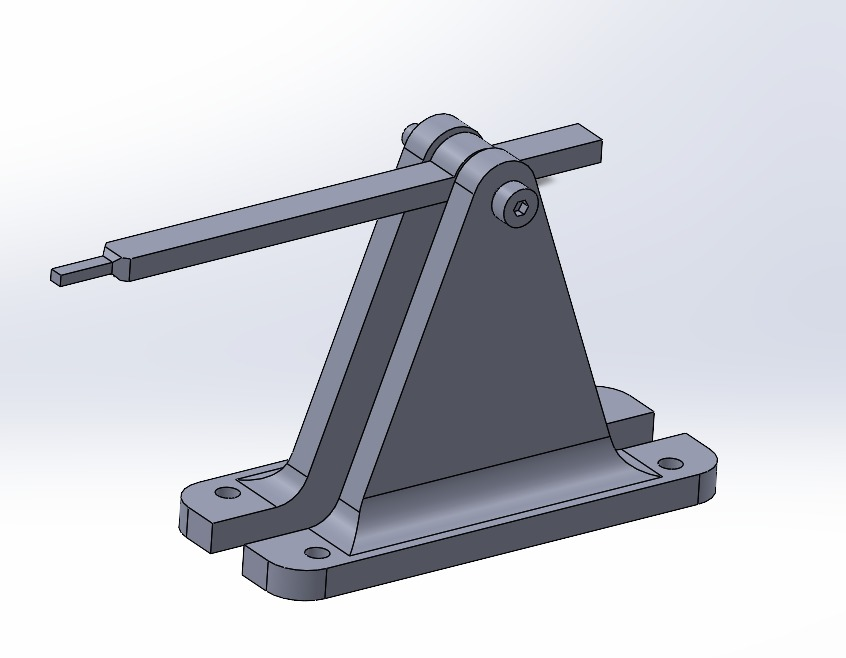
\includegraphics[width=.72\textwidth]{prototype/estrutura.jpg}
  \label{fig:prototipo3d}
  \fonte{Elaborado pelos autores (2026).}
\end{figure}

\begin{figure}[htbp]
  \centering
  \caption{Primeira montagem eletrônica: Blue Pill e driver DRV8871 em placa ilhada.}
  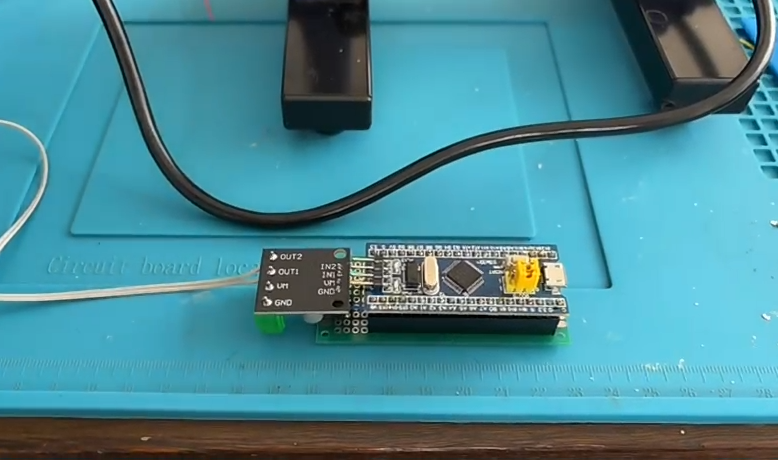
\includegraphics[width=.72\textwidth]{prototype/eletronica.png}
  \label{fig:hardware}
  \fonte{Elaborado pelos autores (2026).}
\end{figure}

\section{OBJETIVOS E ESCOPO}

O objetivo geral é projetar, construir e avaliar uma malha de estabilização angular com FreeRTOS no STM32F103, mantendo a haste próxima de $0^\circ$ e demonstrando a aplicação do RTOS a um sistema de controle crítico. Como objetivos específicos:

\begin{alineastcc}
 \item justificar a escolha de um sistema crítico e os fundamentos de RTOS e FreeRTOS que sustentam o projeto;
 \item modelar a dinâmica da haste e simulá-la para escolher e comparar controladores;
 \item montar o protótipo e documentar materiais, ligações e configuração do microcontrolador de forma replicável;
 \item organizar a malha de controle (aquisição, filtragem, PID e acionamento) em uma tarefa periódica de maior prioridade e os comandos e a telemetria em tarefas de menor prioridade, com semáforo, \textit{mutexes} e fila;
 \item tratar o ruído do MPU6050 com filtro complementar e evitar o \textit{windup} da ação integral;
 \item avaliar o equilíbrio da haste e o desempenho temporal do controle.
\end{alineastcc}

O estudo abrange um eixo de rotação e um único atuador, com referência em $0^\circ$ (horizontal). O PID foi adotado por sua estrutura simples e porque uma implementação anterior em Arduino, sem RTOS, já havia equilibrado a haste de forma qualitativa. Essa observação motivou o projeto, mas não é medida de desempenho.

\clearpage
\section{CRONOGRAMA GERAL}
A Figura~\ref{fig:cronograma} apresenta o cronograma de Gantt elaborado pelo grupo para o período de agosto a dezembro de 2026. A imagem reúne as atividades, suas durações e os marcos de entrega previstos.
\begin{figure}[H]
\centering
\caption{Cronograma de Gantt do projeto.}\label{fig:cronograma}
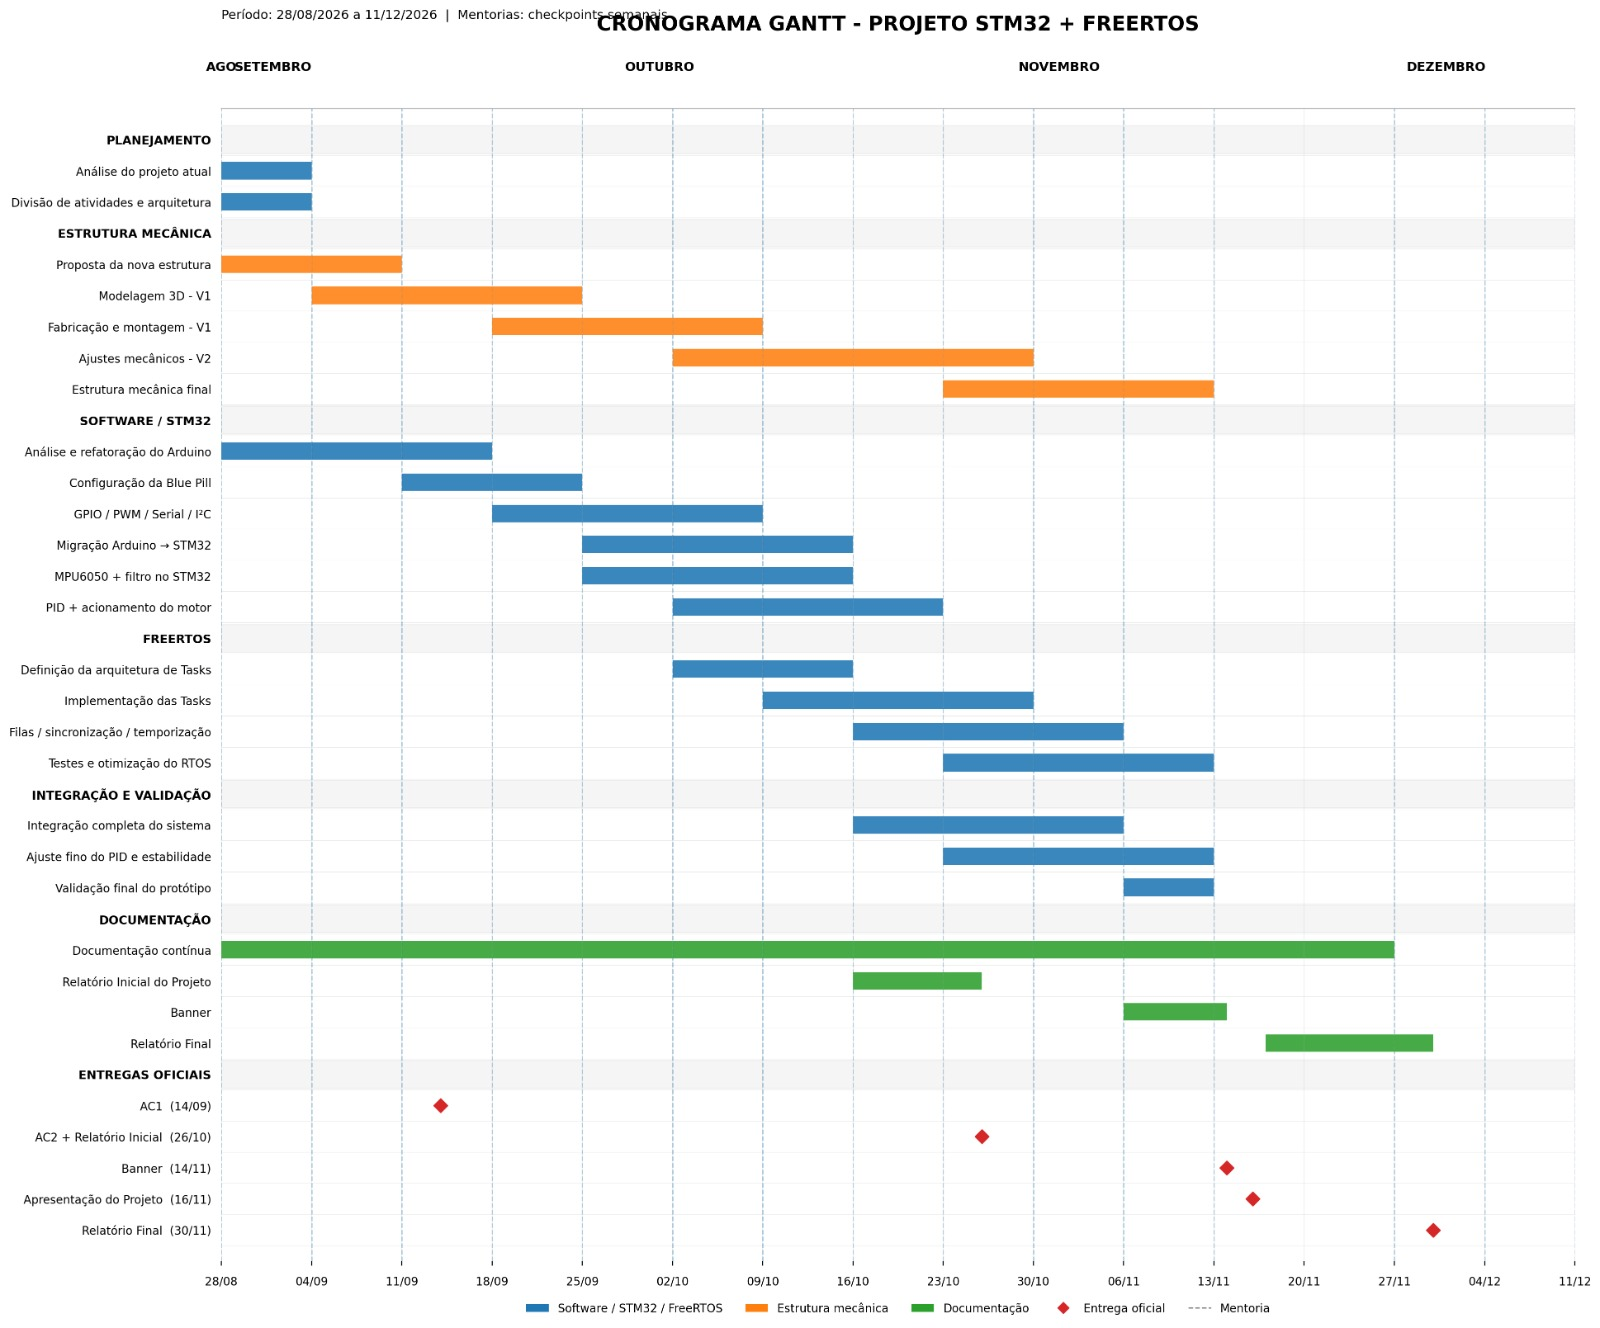
\includegraphics[width=\textwidth]{cronograma-gantt.jpg}
\fonte{Elaborado pelos autores (2026).}
\end{figure}

\clearpage
\chapter{SISTEMAS CRÍTICOS, RTOS E FREERTOS}\label{cap:rtos}

\section{POR QUE UM SISTEMA CRÍTICO}

Um sistema de tempo real é aquele cujo comportamento correto depende não só do resultado, mas do instante em que ele é produzido. Em sistemas de tempo real \textit{hard}, perder um prazo equivale a uma falha; em sistemas \textit{soft}, a perda apenas degrada o desempenho \cite{buttazzo2011,burns2009}. A malha de atitude de um multirrotor se aproxima do primeiro caso: o veículo é instável em malha aberta, e uma sequência de atualizações atrasadas deixa o ângulo crescer até a queda.

A haste 1DOF reproduz essa característica. Com o motor desligado, a haste cai e repousa em cerca de $-38^\circ$ (valor lido pelo sensor); perto da horizontal não há torque restaurador e a planta se comporta como um integrador duplo, de modo que o empuxo precisa ser corrigido continuamente. Dois fatos medidos na bancada tornam o prazo concreto: o empuxo responde ao comando com atraso de cerca de 58~ms (Capítulo~\ref{cap:processo}) e a haste acelera cerca de $300^\circ/\mathrm{s}^2$ para cada 1\% de PWM. Se o controle ficar parado por algumas dezenas de milissegundos, a haste já percorreu uma fração relevante da faixa de operação. O período de 5~ms escolhido é cerca de doze vezes menor que o atraso do atuador. Se as atualizações atrasarem, a malha perde margem de fase e passa a oscilar.

A política implementada é simples: uma leitura inválida pula o ciclo e mantém a saída anterior; se o sensor fica 50~ms sem responder (10 ciclos seguidos), o motor é desligado. O firmware não descarta amostras por idade; o atraso da malha é tratado na análise temporal (Seção~\ref{sec:temporal}). Classificar o sistema como tempo real \textit{hard} ou \textit{firm} depende do que acontece quando um prazo é perdido. Aqui, o pior caso é a haste cair, sem risco para pessoas; por isso o prazo é tratado como crítico para o desempenho, e não para a segurança.

Controladores de voo reais seguem a mesma lógica: \citeonline{rico2022} propõem um controlador de voo com um RTOS simplificado, de escalonador híbrido (ordem de chegada e prazo mais próximo, com prioridade dinâmica), validado por testes de escalonabilidade e por dados de voo, e com a unidade de sensores isolada da vibração. Este trabalho usa o escalonamento por prioridades fixas do FreeRTOS, que basta para uma malha crítica e duas tarefas de apoio.

\section{SISTEMAS OPERACIONAIS DE TEMPO REAL}

Um sistema operacional organiza a execução dos programas e o acesso aos recursos do processador. Em um sistema embarcado, cada tarefa é um trecho de código que roda como se tivesse o processador só para si; o escalonador decide qual tarefa executa, e as interrupções avisam que algo aconteceu fora do processador. Um RTOS acrescenta previsibilidade: a tarefa pronta de maior prioridade sempre recebe o processador (preempção por prioridades fixas), e as primitivas de sincronização têm tempo limitado \cite{barry2016}. A previsibilidade, entretanto, depende da análise conjunta dos tempos de execução, das prioridades e dos bloqueios da aplicação \cite{burns2009,buttazzo2011}.

\section{O FREERTOS}

O FreeRTOS é um núcleo de código aberto para microcontroladores que oferece tarefas, filas, semáforos, \textit{mutexes}, temporizadores de software e gerenciamento de memória \cite{freertosmanual,barry2016}. Os conceitos usados neste trabalho são:

\begin{itemize}
 \item \textbf{Tarefas e prioridades:} cada tarefa é uma função com laço infinito e pilha própria; maior número significa maior prioridade.
 \item \textbf{Semáforo binário:} sinaliza um evento. A interrupção do temporizador libera o semáforo e a tarefa de controle, bloqueada à espera, acorda (processamento diferido da interrupção).
 \item \textbf{Fila:} transfere cópias de dados entre uma interrupção ou tarefa produtora e uma tarefa consumidora. Usada para os bytes recebidos pela serial.
 \item \textbf{\textit{Mutex} com herança de prioridade:} garante exclusão mútua em dados compartilhados; se uma tarefa de maior prioridade espera, a proprietária herda temporariamente a prioridade, o que limita a inversão de prioridade \cite{barry2016}.
 \item \textbf{Funções \texttt{FromISR}:} únicas permitidas dentro de interrupções. No Cortex-M3 as interrupções que as chamam precisam ter prioridade numérica igual ou maior que o limite configurado, pois no NVIC números menores são mais urgentes \cite{freertoscortex}.
\end{itemize}

O STM32F103 usa um núcleo Arm Cortex-M3 de até 72~MHz, sem unidade de ponto flutuante, com 20~kB de SRAM e 64~kB de Flash declarados (a placa utilizada reporta 128~kB) \cite{stm32f103ds}. Por isso as contas com \texttt{float} são feitas em software e pesam no tempo de execução.

\section{FUNDAMENTOS DE CONTROLE E ESTIMAÇÃO}

\subsection{Estimação do ângulo: acelerômetro, giroscópio e filtro complementar}

O acelerômetro mede a direção da gravidade e permite obter o ângulo absoluto por \texttt{atan2} \cite{nxpan3461}, mas é sensível a acelerações e vibrações. O giroscópio mede a velocidade angular e, integrado, fornece um ângulo suave, porém com deriva por causa do viés. O filtro complementar combina os dois: o giroscópio domina no curto prazo e o acelerômetro corrige a deriva no longo prazo \cite{colton2007}.
\begin{equation}
 \hat\theta[k]=\alpha\left(\hat\theta[k-1]+T_s\,\omega_g[k]\right)+(1-\alpha)\,\theta_a[k],\qquad \alpha=\frac{\tau_f}{\tau_f+T_s}
\end{equation}
É um filtro de ordem um, de custo desprezível no Cortex-M3 e com um único parâmetro de ajuste, $\tau_f$. No firmware, essa correção muda com o motor: desligado, o acelerômetro acerta o ângulo em poucos segundos; ligado, a correção é lenta, da ordem de 30~s, porque a vibração da hélice atrapalha a leitura (Seções~\ref{sec:ruido} e~\ref{sec:deriva}).

\subsection{PID discreto, derivada na medida e anti-\textit{windup}}

O controlador PID soma uma parcela proporcional ao erro, uma integral do erro e uma derivativa \cite{astrom1995}. Na forma discreta com período $T_s$ e $e=\theta_r-\hat\theta$,
\begin{equation}
 u[k]=K_p\,e[k]+I[k]-K_d\,\dot{\hat\theta}[k],\qquad I[k]=I[k-1]+K_i\,e[k]\,T_s
\end{equation}
A derivada é calculada sobre a medida (aqui, a velocidade do giroscópio) e não sobre o erro, o que evita o pico de saída quando a referência muda \cite{astrom1995}.

O atuador tem limites: o PWM varia de 0 a um máximo, e a hélice só empurra em um sentido. Quando a saída satura, o integrador continua acumulando o erro e, ao voltar à faixa linear, a saída fica presa no extremo até o integrador descarregar. Esse fenômeno é o \textit{integrator windup} \cite{astrom1989}. As técnicas clássicas são limitar o integrador (\textit{clamping}) e a integração condicional, que suspende a integração enquanto a saída está saturada e o erro a empurra mais para dentro da saturação \cite{astrom1989,astrom2008}. O firmware usa a integração condicional; o Capítulo~\ref{cap:processo} compara as alternativas por simulação.

\clearpage
\chapter{MODELAGEM E SIMULAÇÃO}\label{cap:processo}

\section{MODELO FÍSICO}

A planta é uma haste rígida que gira em torno de um eixo fixo. O empuxo $F$ é a entrada e o ângulo $\theta$ em relação à horizontal (positivo quando o motor sobe) é a variável regulada. A soma dos torques sobre o pivô fornece a segunda lei de Newton para a rotação, na mesma forma usada em plataformas 1DOF descritas na literatura \cite{mane2019,cuero2020,uyar2024}:
\begin{equation}
 J\ddot\theta=l_mF-g\,S_m\cos\theta-b\dot\theta+\tau_d
 \label{eq:modelo}
\end{equation}
em que $J$ é o momento de inércia em torno do pivô, $l_m$ o braço do motor, $S_m$ o momento estático das massas em relação ao pivô (positivo do lado do motor), $b$ o atrito viscoso e $\tau_d$ um torque externo. O empuxo responde ao comando $u$ (PWM) com dinâmica de primeira ordem de constante $\tau_m$:
\begin{equation}
 \tau_m\dot F=F_{\max}\,u-F
\end{equation}
Na horizontal o termo $\cos\theta$ tem derivada nula, de modo que, em torno de $\theta=0$, a planta se comporta como um integrador duplo com atraso de primeira ordem. Isso explica por que um controle apenas proporcional oscila e por que a ação derivativa é indispensável.

\section{IDENTIFICAÇÃO NA BANCADA}

Não há dados confiáveis de massa e empuxo do kit. Em vez de estimá-los, a planta foi identificada com o próprio firmware, a partir dos registros de ângulo e saída gravados na RAM em 6 de outubro de 2026. O modelo reduzido da Equação~\ref{eq:modelo}, escrito direto em graus e em porcentagem de PWM, foi ajustado a dois registros feitos com ganhos diferentes:
\begin{table}[htbp]
\centering\caption{Parâmetros da planta identificados na bancada.}\label{tab:parametros}
\begin{tabularx}{\textwidth}{Xrl}
\hline\textbf{Parâmetro} & \textbf{Valor} & \textbf{Origem}\\\hline
Ganho do atuador & $\approx 300^\circ/\mathrm{s}^2$ por 1\% de PWM & ajuste ao registro\\
PWM para pairar & $\approx 20{,}2\%$ (16 a 23\% nos registros anteriores) & partida de 02/11/2026\\
Atraso do empuxo $\tau_m$ & $\approx 58$ ms & ajuste ao registro\\
Atraso puro (filtro do sensor e amostragem) & $\approx 9$ ms & ajuste ao registro\\
Repouso (haste caída) & $\approx -38^\circ$ & leitura do sensor\\
Limite de saída & 32\% & projeto (Seção~\ref{sec:potencia})\\\hline
\end{tabularx}
\fonte{Elaborado pelos autores (2026), com \texttt{firmware/tools/arm\_margins.py} e \texttt{firmware/tools/arm\_tune.py}.}
\end{table}
A frequência de oscilação prevista pelo modelo para os ganhos usados na segunda rodada foi 18,4~rad/s; a medida na bancada foi 18~rad/s, o que sustenta a identificação. O modelo é de pequenos sinais em torno do ponto de pairar e não representa zona morta nem a não linearidade da curva PWM--empuxo. Massa, inércia e braços não foram medidos; a pesagem das peças permanece como trabalho futuro.

\section{CONTROLE E MARGENS DE ESTABILIDADE}

Com a planta identificada, a margem de fase foi calculada pela resposta em frequência da malha (PID com derivada filtrada, integrador duplo, atraso de empuxo e atraso puro). Com os ganhos iniciais ($K_p=1{,}0$, $K_i=0{,}5$, $K_d=0{,}15$), a haste ficou em ciclo-limite entre $-10{,}8^\circ$ e $+5{,}4^\circ$, com a saída batendo nos limites. Com $0{,}30/0{,}15/0{,}09$, a margem de fase era de só $3{,}6^\circ$ e a haste oscilou $\pm3{,}7^\circ$. Os ganhos de projeto, $K_p=0{,}06$, $K_i=0{,}05$ e $K_d=0{,}04$, com filtro da derivada de 5~ms, foram escolhidos para ter cerca de $43^\circ$ de margem de fase nominal e pelo menos $33^\circ$ com o ganho do atuador entre 120 e $380^\circ/\mathrm{s}^2$ por 1\% e o atraso entre 45 e 75~ms. Depois, o refino na bancada subiu $K_i$ para 0,08 (Capítulo~\ref{cap:refino}). A lição é que, com atraso de empuxo de dezenas de milissegundos, ganho alto produz oscilação, e não precisão.

\section{SIMULAÇÃO}

O simulador (\texttt{report/simulation/sim\_1dof.py}, Python com NumPy e Matplotlib) integra o modelo identificado com passo de 5~ms e reproduz o PID do firmware linha a linha: derivada na medida, filtro da derivada, limites de 10\% a 32\%, rampa de saída de 300\%/s e integrador iniciado em 16\% \footnote{Uma versão anterior do trabalho usava um simulador em Drake com parâmetros estimados; ela foi substituída por este modelo, que usa a planta identificada. Os resultados antigos não são reutilizados.}. Esse modelo também existe em C (\texttt{firmware/tests/sim\_control.c}), que compila o \texttt{control.c}, o \texttt{pid.c} e o \texttt{angle\_filter.c} do próprio firmware, de modo que a lógica embarcada é testada no computador.

Usando o PWM de pairar medido na bancada (20,2\%), a simulação leva a haste do repouso, a $-38^\circ$, até a faixa de $\pm2^\circ$ em torno do alvo em cerca de 5,7~s, com sobressinal de cerca de $0{,}3^\circ$ (Figura~\ref{fig:partida}). Na bancada, a mesma partida levou 6,6~s (Capítulo~\ref{cap:resultados}). A subida lenta decorre dos ganhos baixos: o integrador, iniciado em 16\%, é quem sustenta a haste.
\begin{figure}[htbp]
\centering\caption{Partida simulada a partir do repouso, com os ganhos de projeto.}\label{fig:partida}
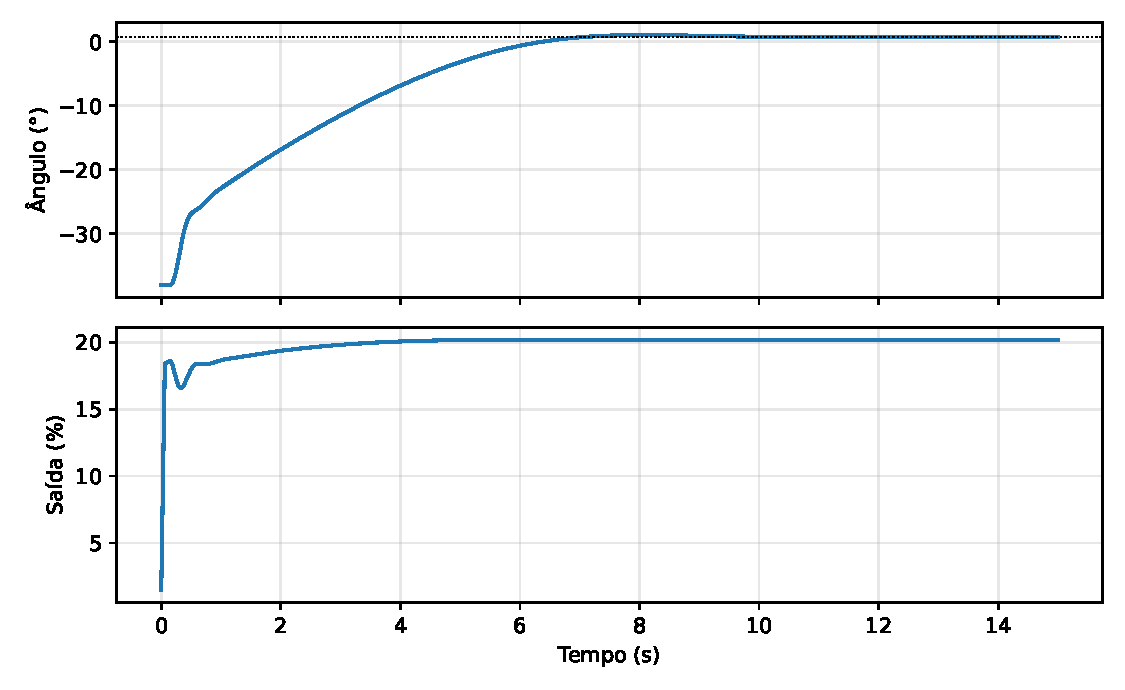
\includegraphics[width=.85\textwidth]{results/partida.pdf}
\fonte{Elaborado pelos autores (2026), simulação com a planta identificada.}
\end{figure}

\section{POR QUE O ANTI-\textit{WINDUP}}\label{sec:antiwindup}

Para isolar o efeito, a simulação segura a haste $25^\circ$ acima do alvo durante 5~s (como uma mão que a impede de se mover) e depois a solta. Durante a retenção o erro é negativo e constante; um integrador sem proteção desce sem limite e, ao soltar, a saída fica abaixo da necessária para pairar por muito tempo. Foram comparadas três versões: integrador sem proteção, integrador apenas limitado a $[0;32]\%$ e integração condicional (a do firmware), cada uma com os ganhos iniciais e com os de projeto. A simulação supõe um batente superior em $+60^\circ$, fora da faixa de interesse.
\begin{table}[htbp]
\centering\caption{Tempo para a haste voltar a $\pm2^\circ$ do alvo depois de solta (simulação).}\label{tab:windup}
\begin{tabularx}{\textwidth}{Xrr}
\hline\textbf{Estratégia} & \textbf{Ganhos iniciais} & \textbf{Ganhos de projeto}\\
 & ($1{,}0/0{,}5/0{,}15$) & ($0{,}06/0{,}05/0{,}04$)\\\hline
Sem proteção & 7,28 s & 7,34 s\\
Apenas limita o integrador & 4,90 s & 7,34 s\\
Integração condicional (firmware) & 1,01 s & 7,34 s\\\hline
\end{tabularx}
\fonte{Elaborado pelos autores (2026), com \texttt{report/simulation/sim\_1dof.py}.}
\end{table}
Com os ganhos iniciais, altos, o \textit{windup} é grave: o integrador sem proteção chega a $-41{,}5\%$ e a recuperação leva 7,3~s contra 1,0~s com a integração condicional (Figura~\ref{fig:windup}). Com os ganhos de projeto, baixos, a saída não satura na retenção e as três estratégias empatam; o anti-\textit{windup} é então uma proteção que não custa nada e passa a ser decisiva quando o ganho aumenta. O resultado também mostra que, com $K_i$ pequeno, o integrador leva cerca de 7~s para se refazer, o que é compatível com a recuperação lenta observada na bancada depois de um empurrão.
\begin{figure}[htbp]
\centering\caption{Haste retida a $+25^\circ$ por 5~s (faixa cinza) com os ganhos iniciais: efeito do \textit{windup}.}\label{fig:windup}
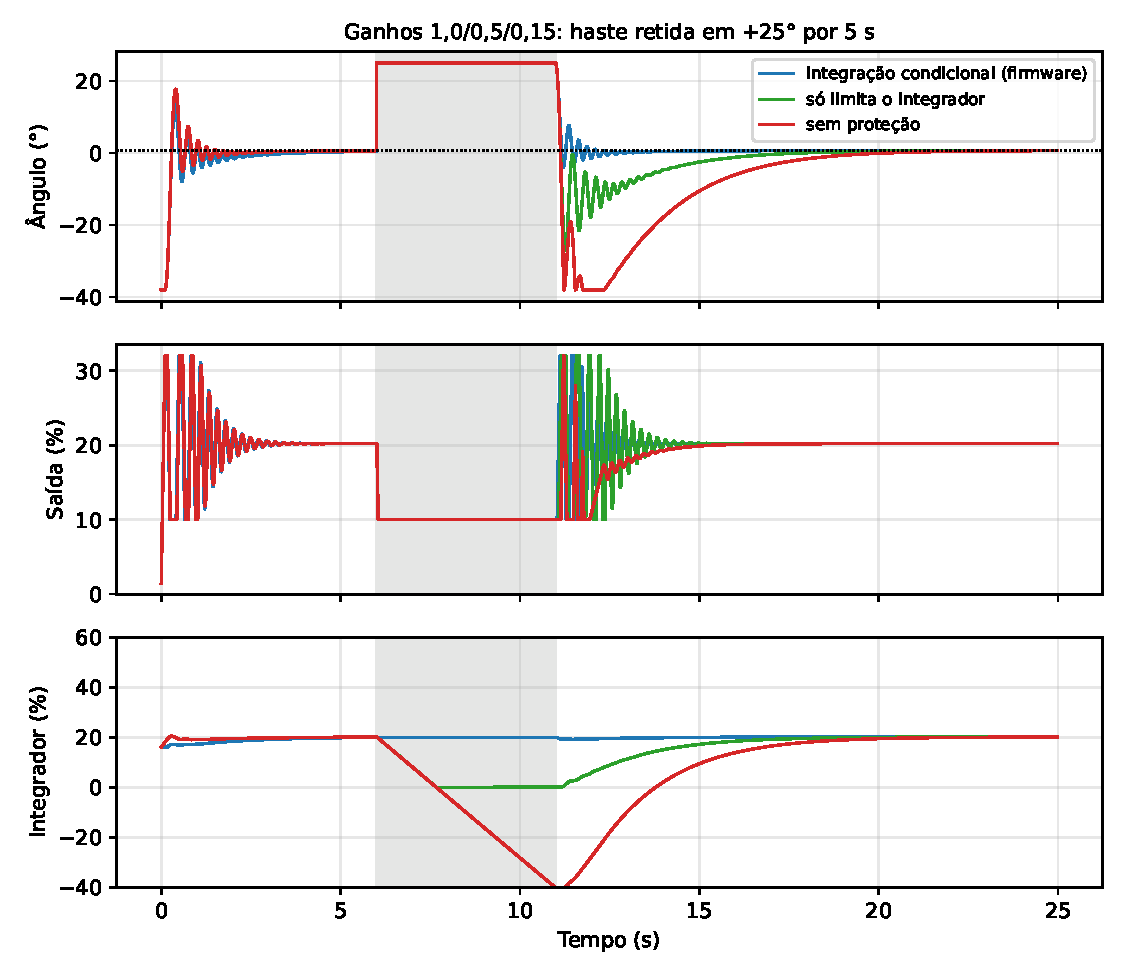
\includegraphics[width=.85\textwidth]{results/windup_ganhos_iniciais.pdf}
\fonte{Elaborado pelos autores (2026), simulação com a planta identificada.}
\end{figure}

\chapter{MATERIAIS, LIGAÇÕES E MONTAGEM}\label{cap:materiais}

\section{LISTA DE MATERIAIS}

\begin{table}[htbp]
\centering\caption{Materiais do protótipo.}\label{tab:materiais}
\begin{tabularx}{\textwidth}{p{4.3cm}X}
\hline\textbf{Item} & \textbf{Função e observações}\\\hline
Blue Pill (STM32F103C8T6) & Microcontrolador Cortex-M3 a 72~MHz, cristal de 8~MHz \cite{stm32f103ds}. Reporta 128~kB de Flash.\\
MPU6050 (módulo) & Acelerômetro e giroscópio de três eixos, ligado por I\textsuperscript{2}C no endereço 0x68 \cite{mpu6050rm}. Alimentado em 3,3~V pelo pino 3V3 da Blue Pill (o módulo aceita de 3,3 a 5~V).\\
Driver DRV8871 (módulo) & Ponte H com limite de corrente; alimentação de 6,5 a 45~V \cite{drv8871ds}. Alimentado direto pelos 12~V.\\
Motor \textit{coreless} 0720 com hélice & Motor de corrente contínua com escovas, de kit Syma: 3,7~V nominais, 7~mm de diâmetro por 20~mm de comprimento e resistência medida de cerca de 2~$\Omega$.\\
Indutor em série com o motor & Indutor toroidal de 220~$\mu$H e 3~A, com fio de cobre enrolado em núcleo toroidal (Figura~\ref{fig:fotos_potencia}), que filtra a corrente pulsada do PWM (Seção~\ref{sec:indutor}). Resistência do enrolamento menor que 0,3~$\Omega$, abaixo do que o multímetro consegue medir.\\
Fonte de 12~V & Alimenta o driver e, pelo BEC, a lógica. O consumo total estimado é inferior a 1~A (motor em torno de 0,4~A e lógica da ordem de 100~mA).\\
BEC 12~V para 5~V & Regulador chaveado que gera os 5~V da Blue Pill.\\
Chave deslizante de 3 terminais & Chave de duas posições ligada em série ao positivo de 5~V entre o BEC e a Blue Pill; um dos terminais fica sem uso. Para cima liga e para baixo desliga (Figura~\ref{fig:alimentacao}).\\
Estrutura & Base de madeira; suporte da haste, haste e caixa da eletrônica impressos em 3D. A massa não foi medida, porque o modelo foi identificado na bancada (Tabela~\ref{tab:parametros}).\\
Parafuso e porca travada & Eixo da haste na base.\\
ST-Link V2 & Gravação e leitura de diagnóstico por SWD.\\\hline
\end{tabularx}
\fonte{Elaborado pelos autores (2026).}
\end{table}

As Figuras~\ref{fig:fotos_estrutura} e~\ref{fig:fotos_potencia} mostram os componentes principais.
\begin{figure}[htbp]
\centering\caption{Estrutura e sensor: (a) suporte da haste impresso em 3D, (b) conjunto do motor com a hélice, (c) hélice e (d) MPU6050 fixado na haste.}\label{fig:fotos_estrutura}
\begin{minipage}[t]{.24\textwidth}\centering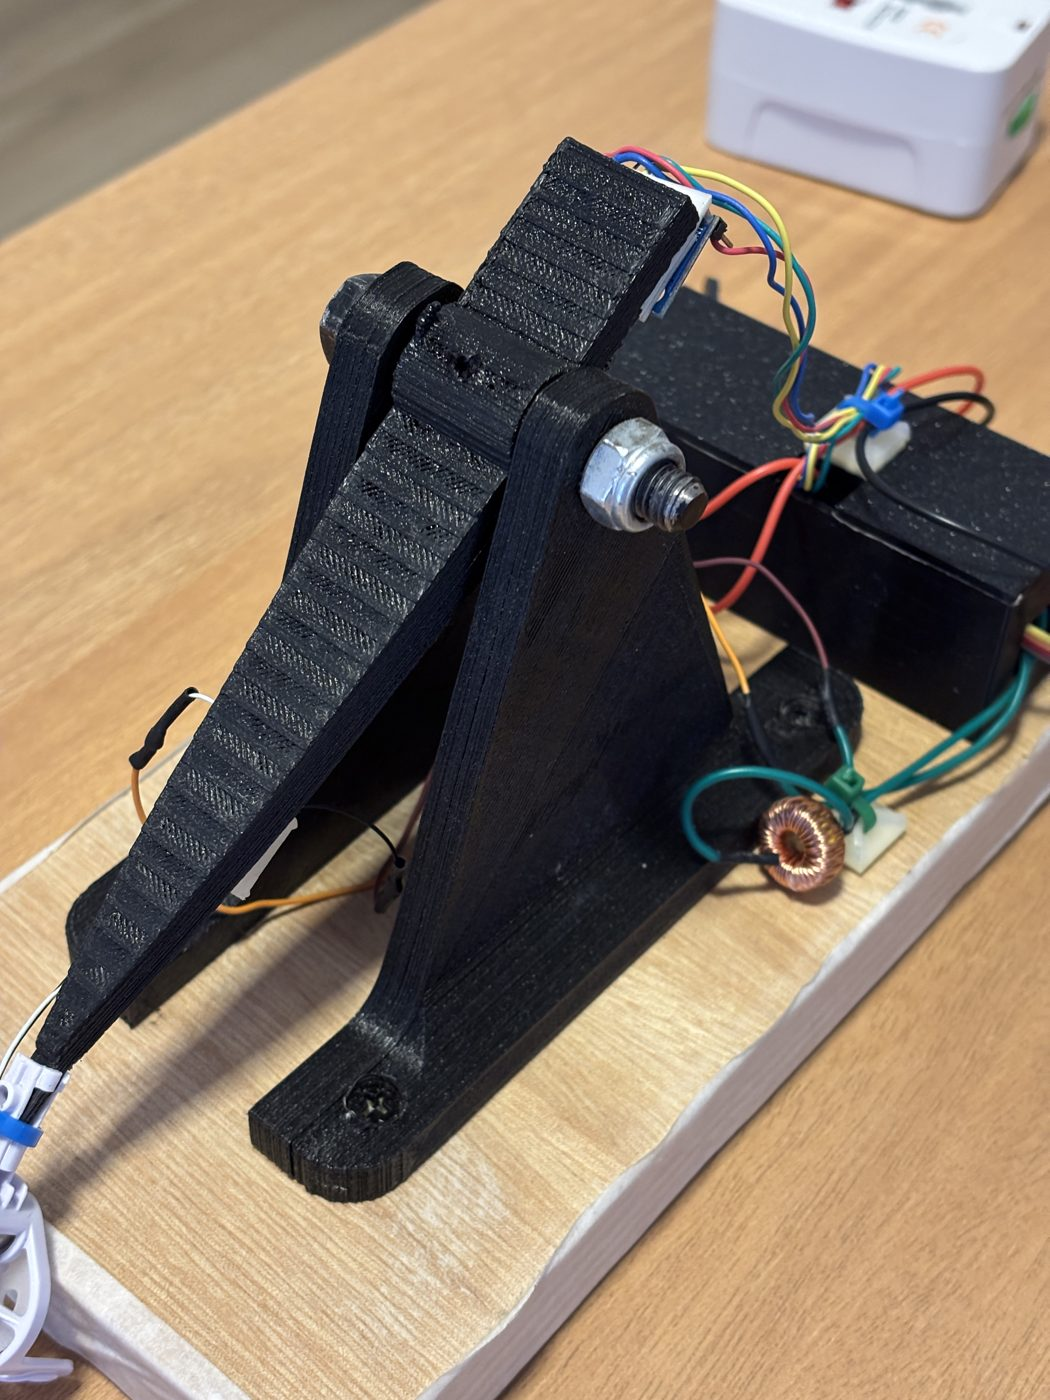
\includegraphics[width=\textwidth]{photos/base_3d.jpg}\\(a)\end{minipage}\hfill
\begin{minipage}[t]{.24\textwidth}\centering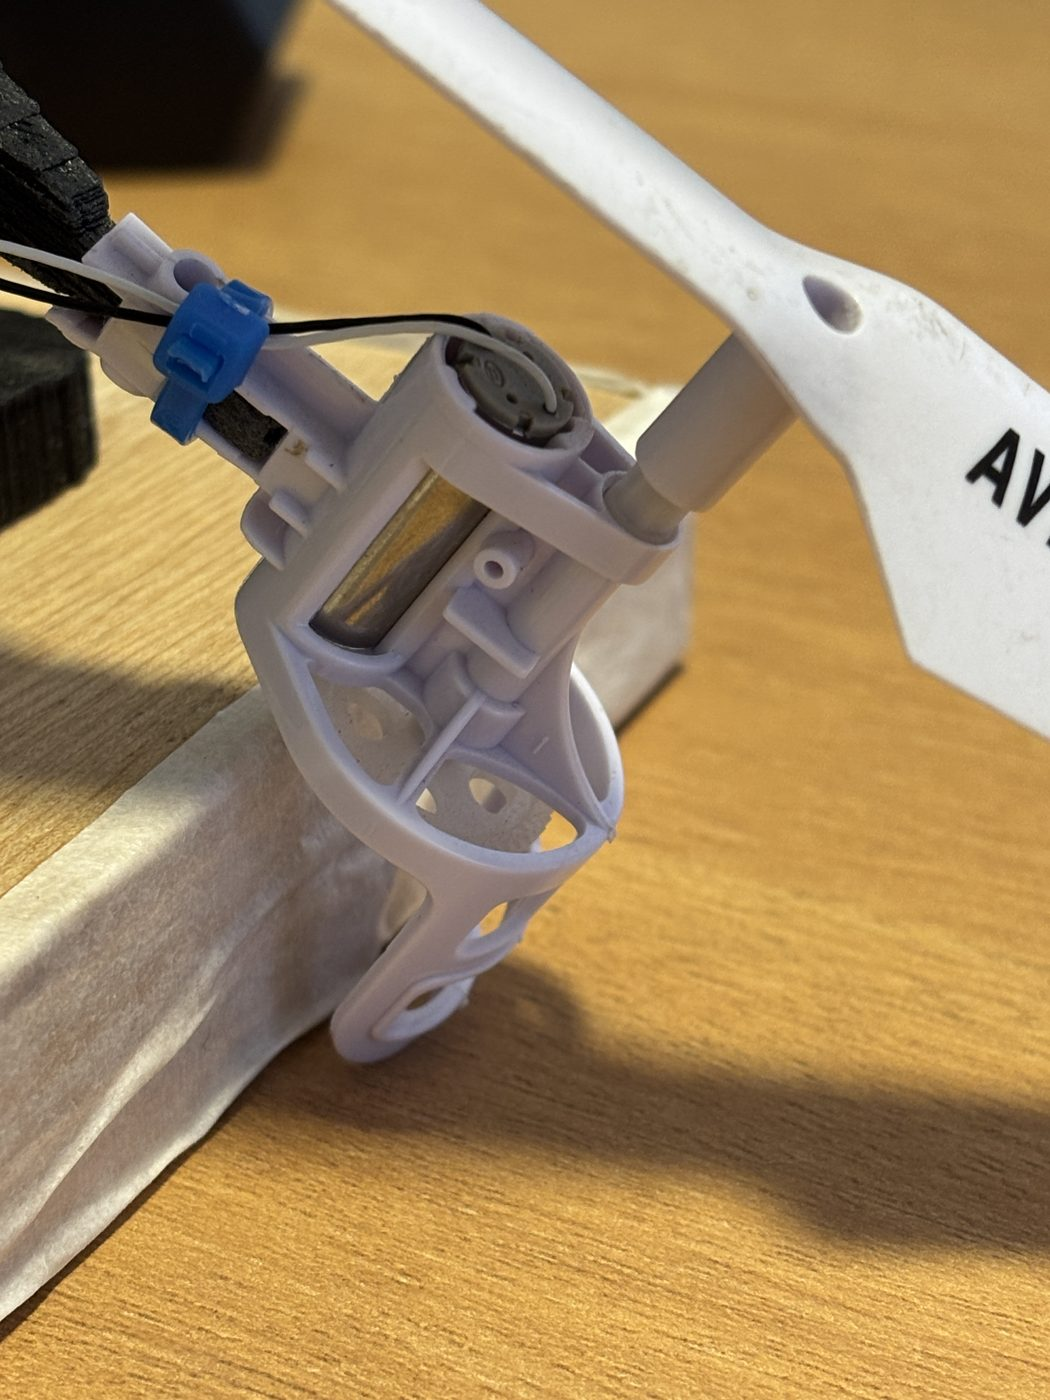
\includegraphics[width=\textwidth]{photos/motor_assembly.jpg}\\(b)\end{minipage}\hfill
\begin{minipage}[t]{.24\textwidth}\centering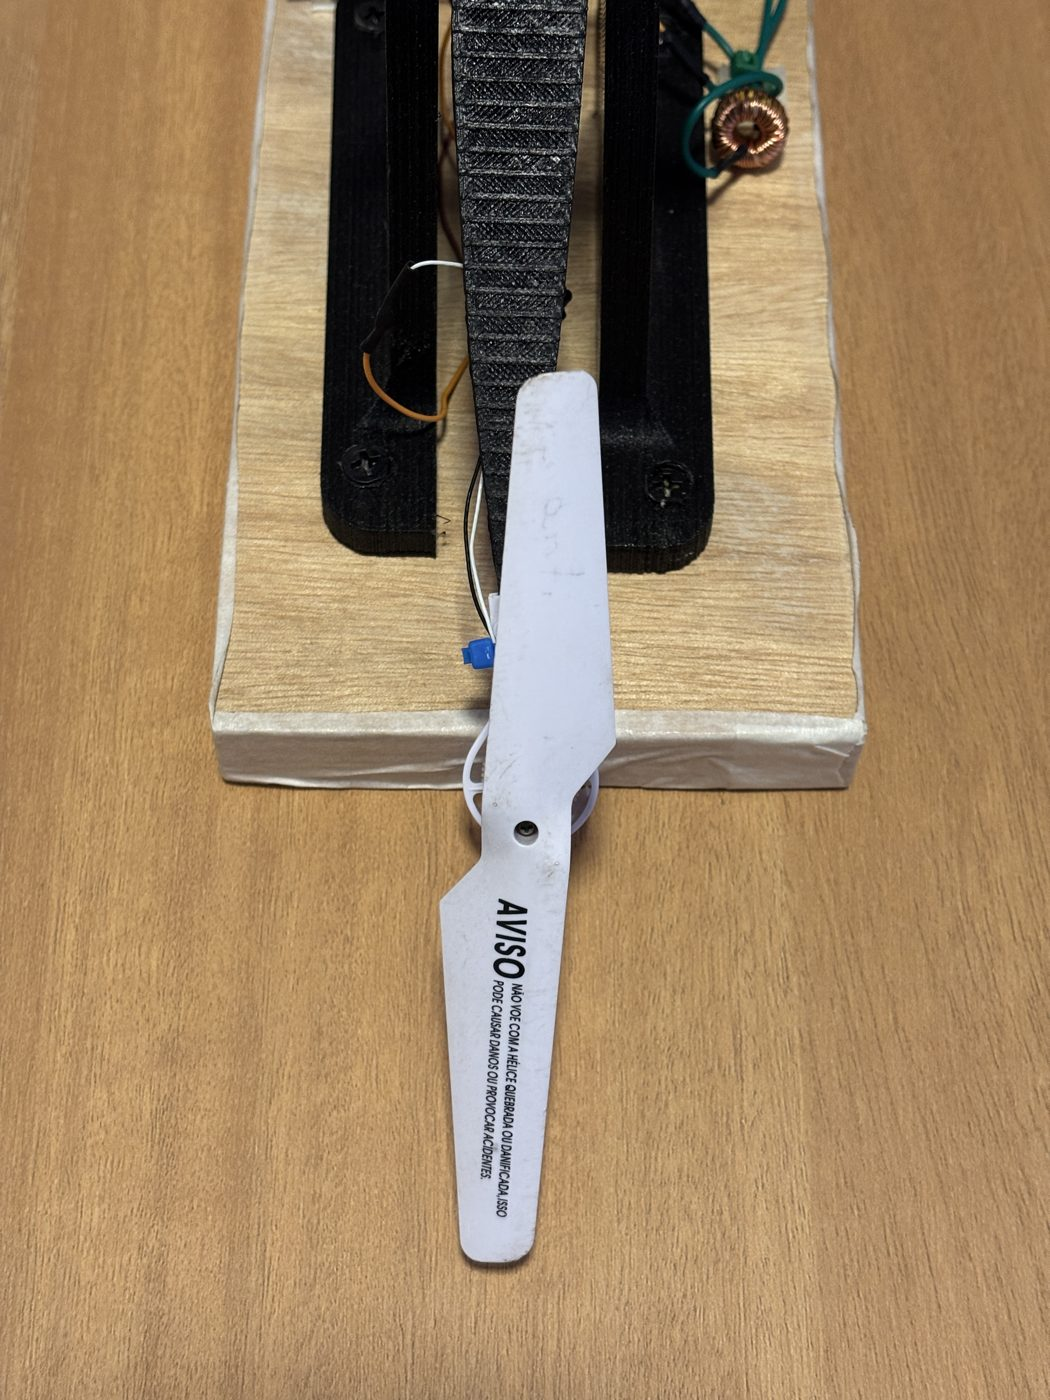
\includegraphics[width=\textwidth]{photos/propeller.jpg}\\(c)\end{minipage}\hfill
\begin{minipage}[t]{.24\textwidth}\centering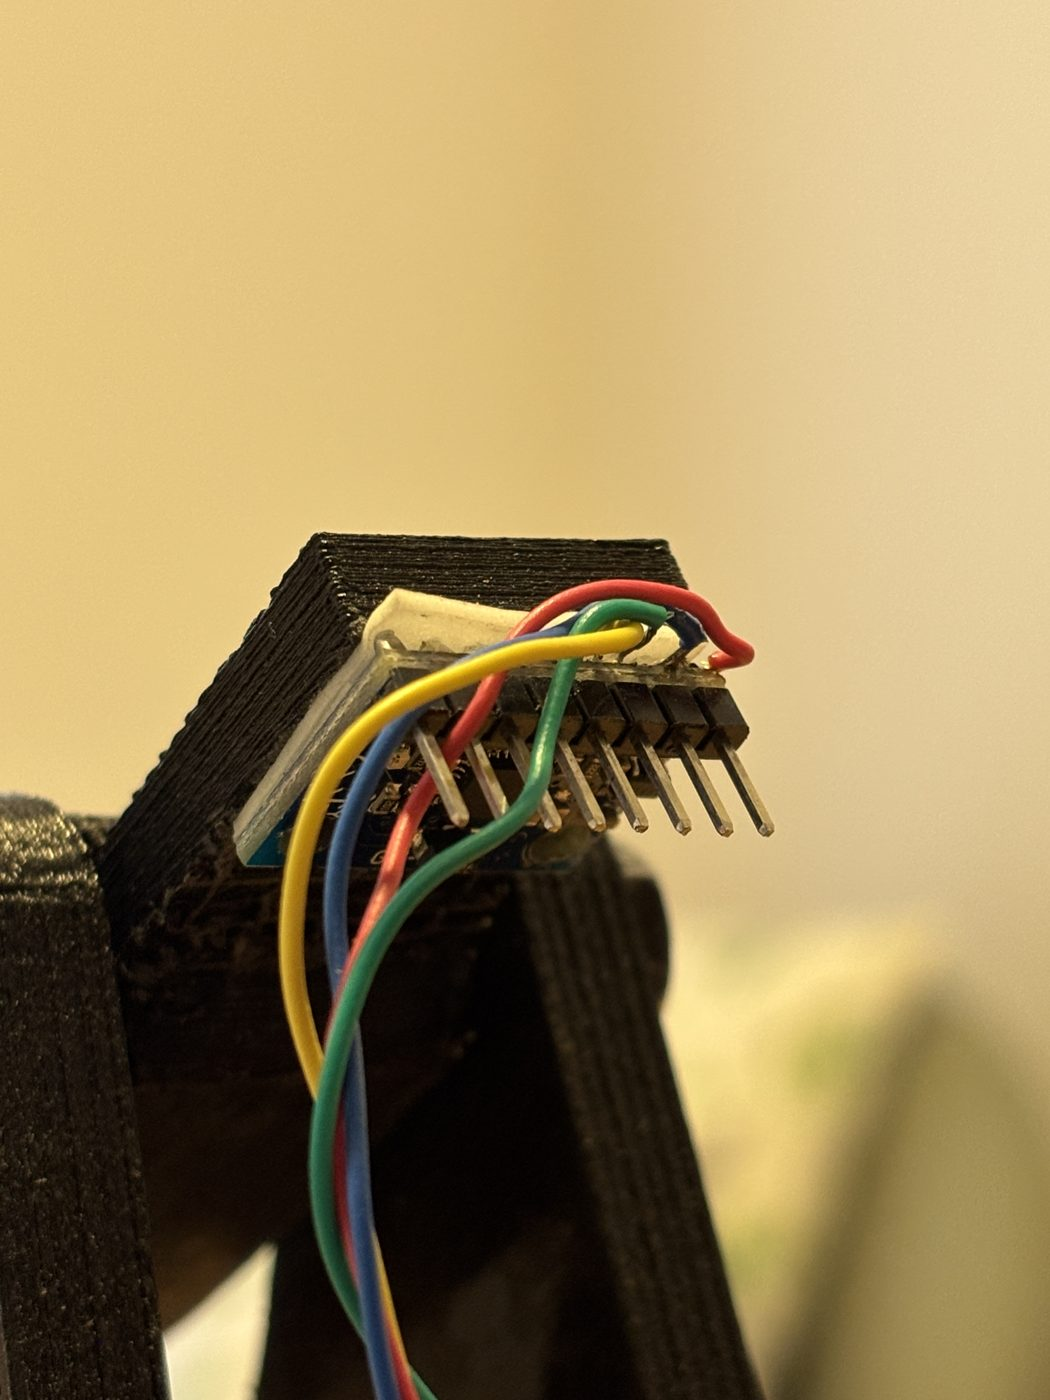
\includegraphics[width=\textwidth]{photos/mpu6050_mount.jpg}\\(d)\end{minipage}
\fonte{Elaborado pelos autores (2026).}
\end{figure}
\begin{figure}[htbp]
\centering\caption{Eletrônica e alimentação: (a) Blue Pill e driver na caixa impressa em 3D, (b) BEC com a saída de 5~V, (c) entrada de 12~V, (d) chave liga/desliga, (e) indutor toroidal de 220~$\mu$H e (f) ST-Link V2.}\label{fig:fotos_potencia}
\begin{minipage}[t]{.32\textwidth}\centering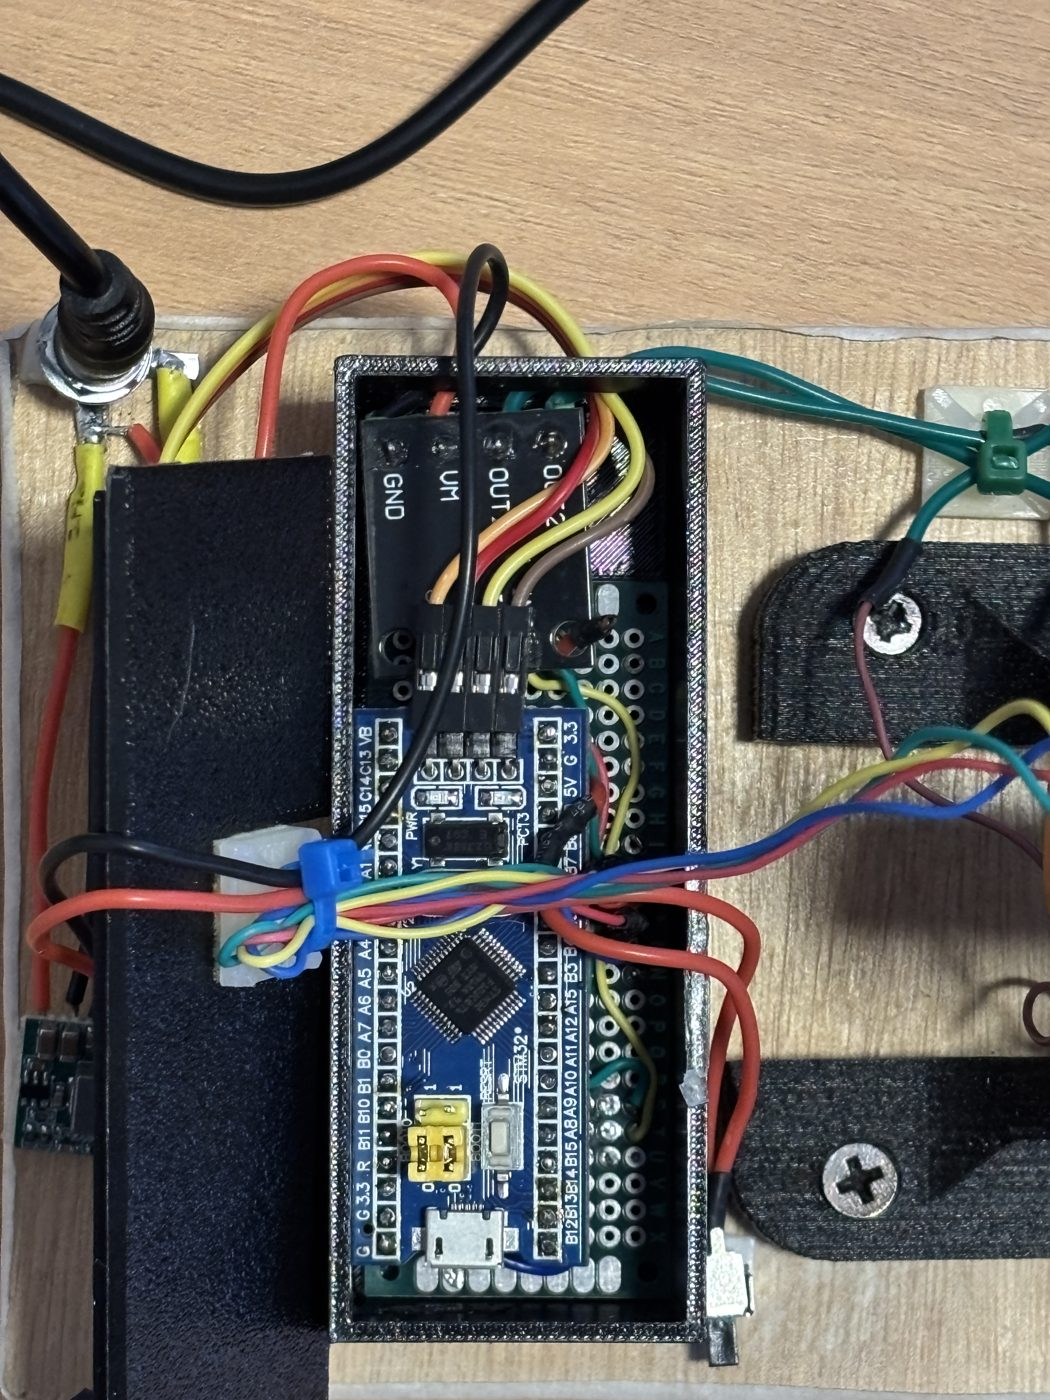
\includegraphics[width=\textwidth]{photos/stm32_driver_box.jpg}\\(a)\end{minipage}\hfill
\begin{minipage}[t]{.32\textwidth}\centering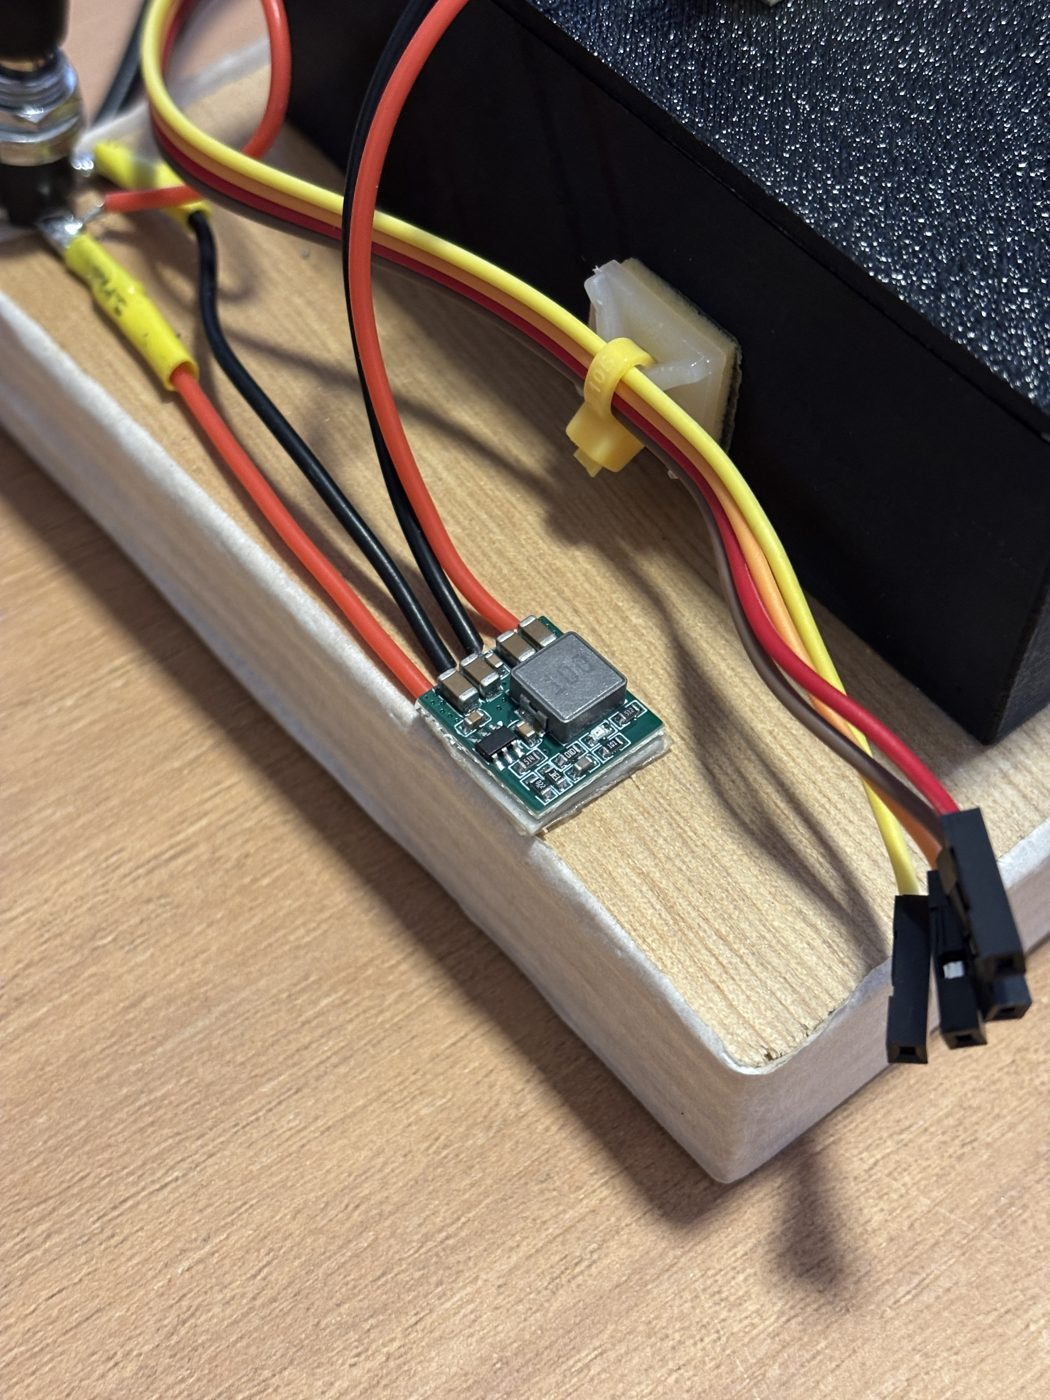
\includegraphics[width=\textwidth]{photos/bec_5v_output.jpg}\\(b)\end{minipage}\hfill
\begin{minipage}[t]{.32\textwidth}\centering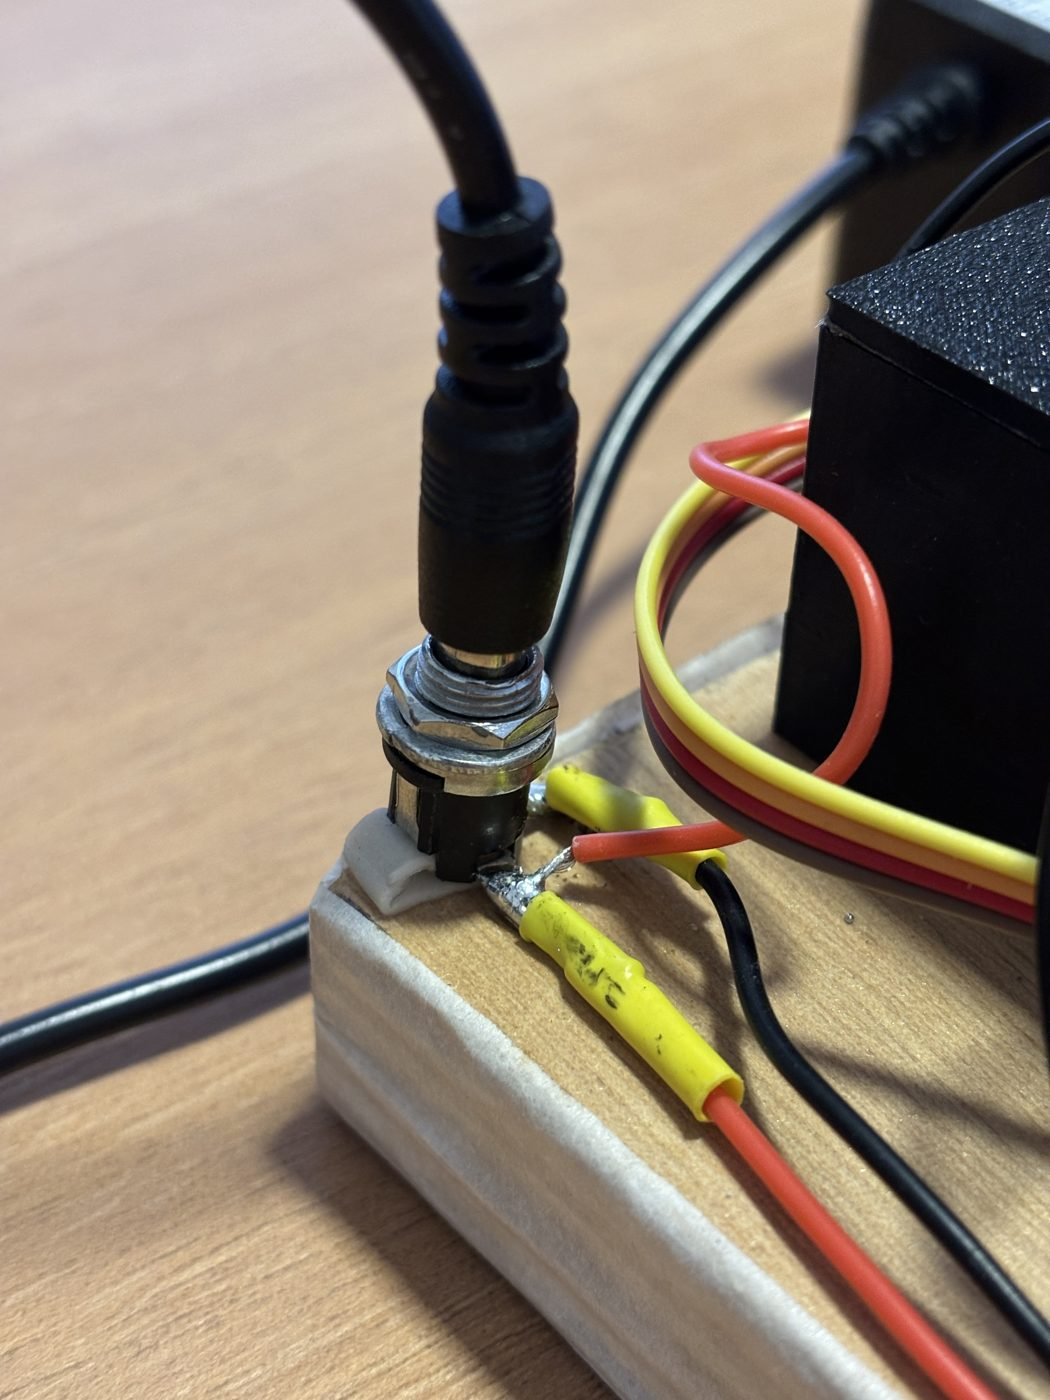
\includegraphics[width=\textwidth]{photos/input_12v.jpg}\\(c)\end{minipage}\\[6pt]
\begin{minipage}[t]{.32\textwidth}\centering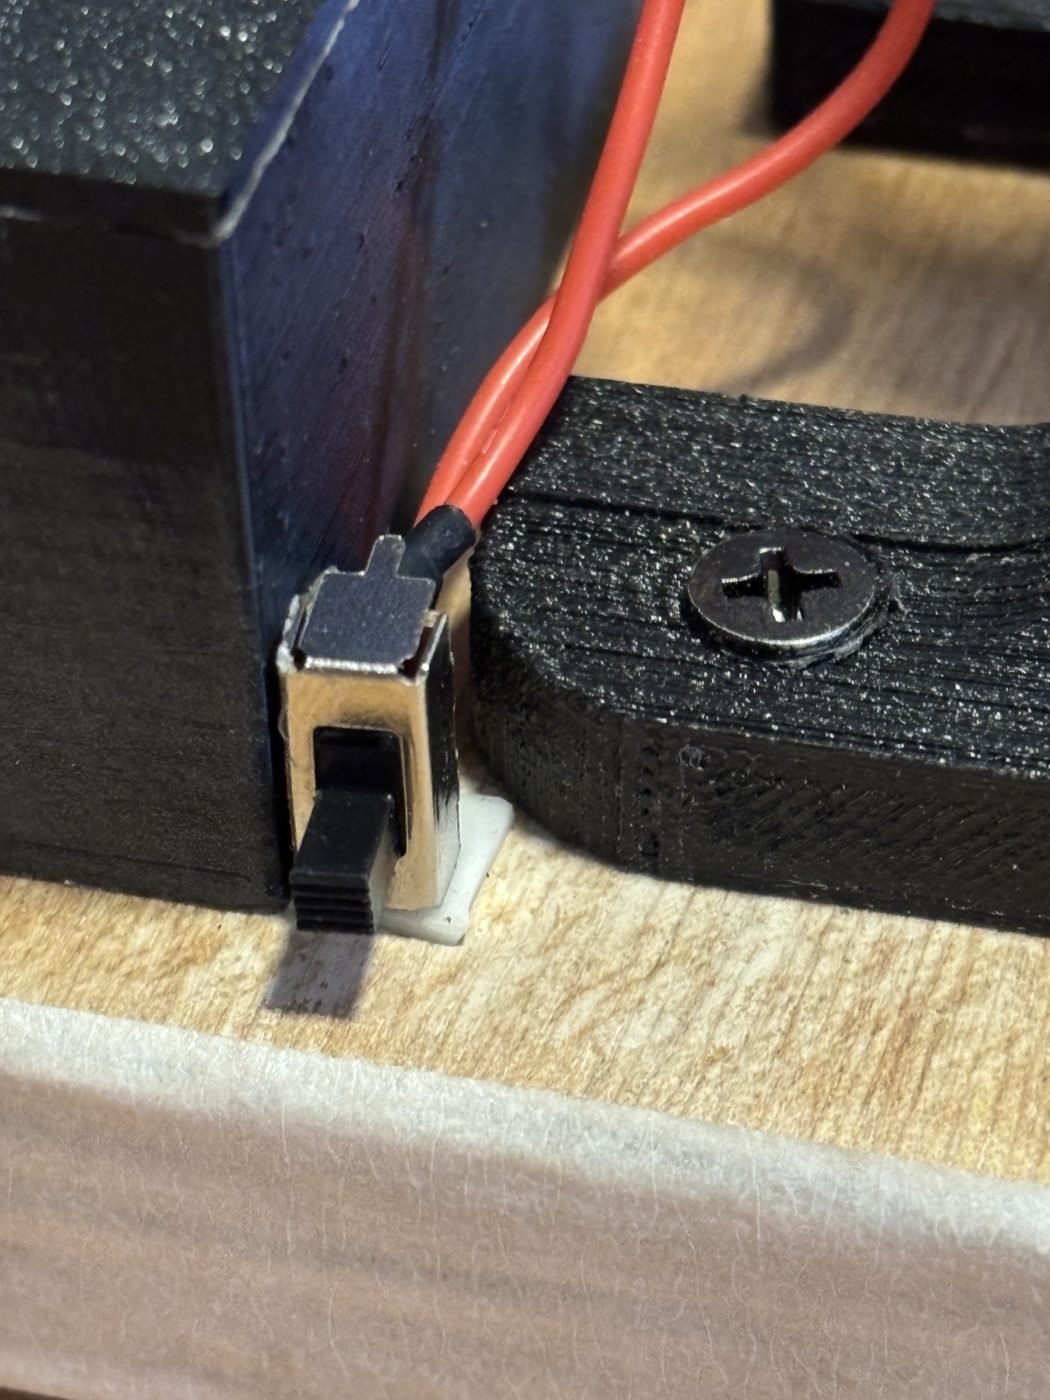
\includegraphics[width=\textwidth]{photos/power_switch.jpg}\\(d)\end{minipage}\hfill
\begin{minipage}[t]{.32\textwidth}\centering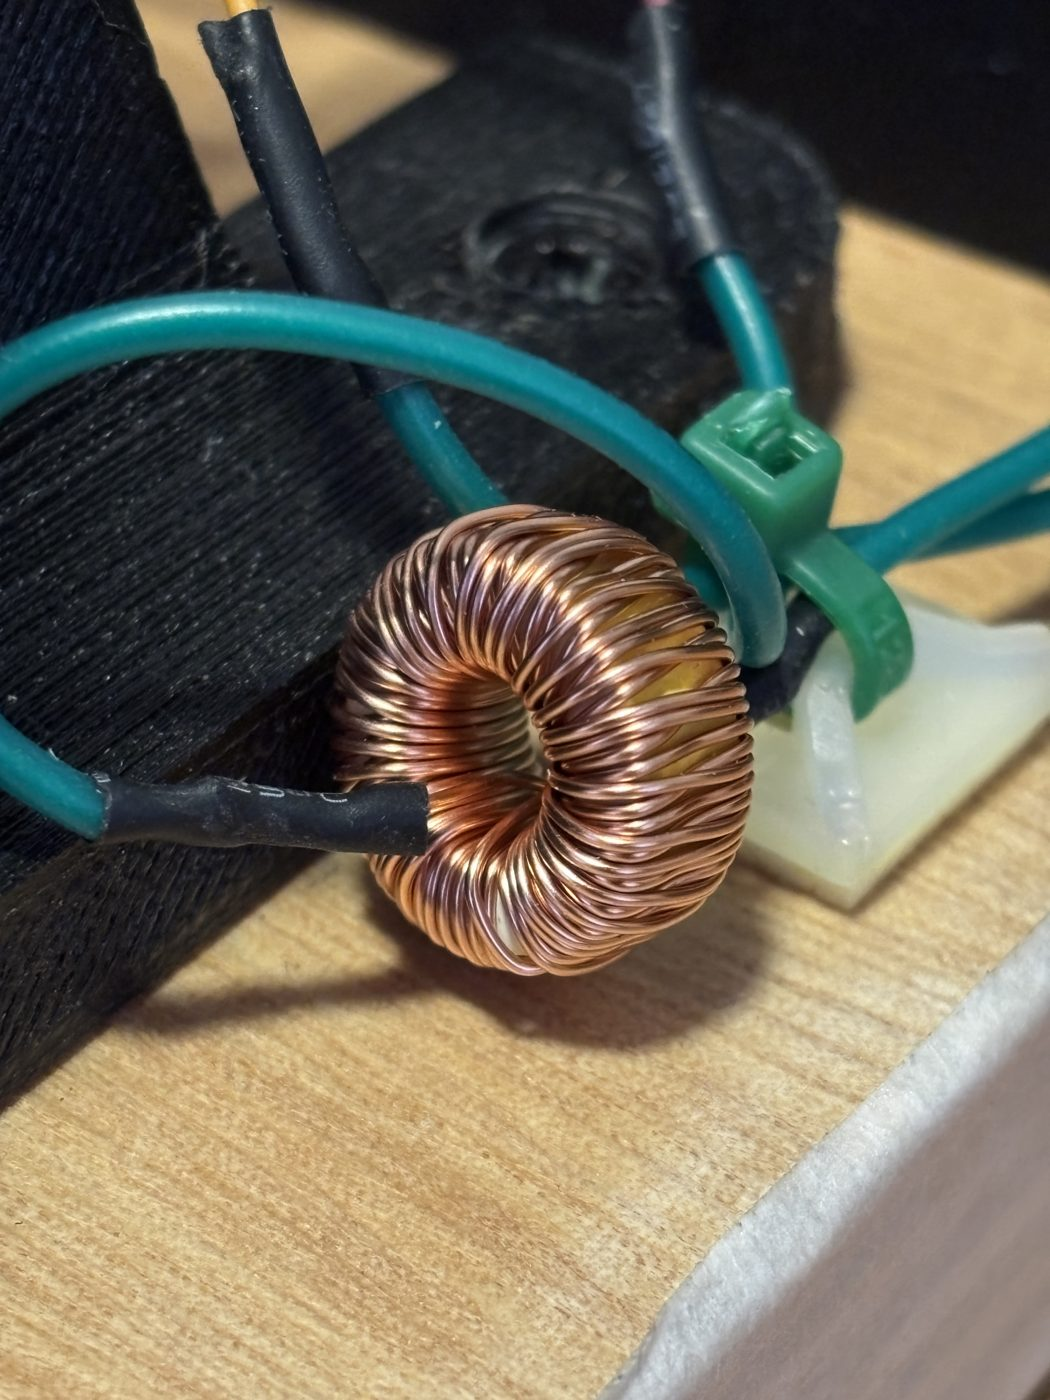
\includegraphics[width=\textwidth]{photos/inductor_toroid.jpg}\\(e)\end{minipage}\hfill
\begin{minipage}[t]{.32\textwidth}\centering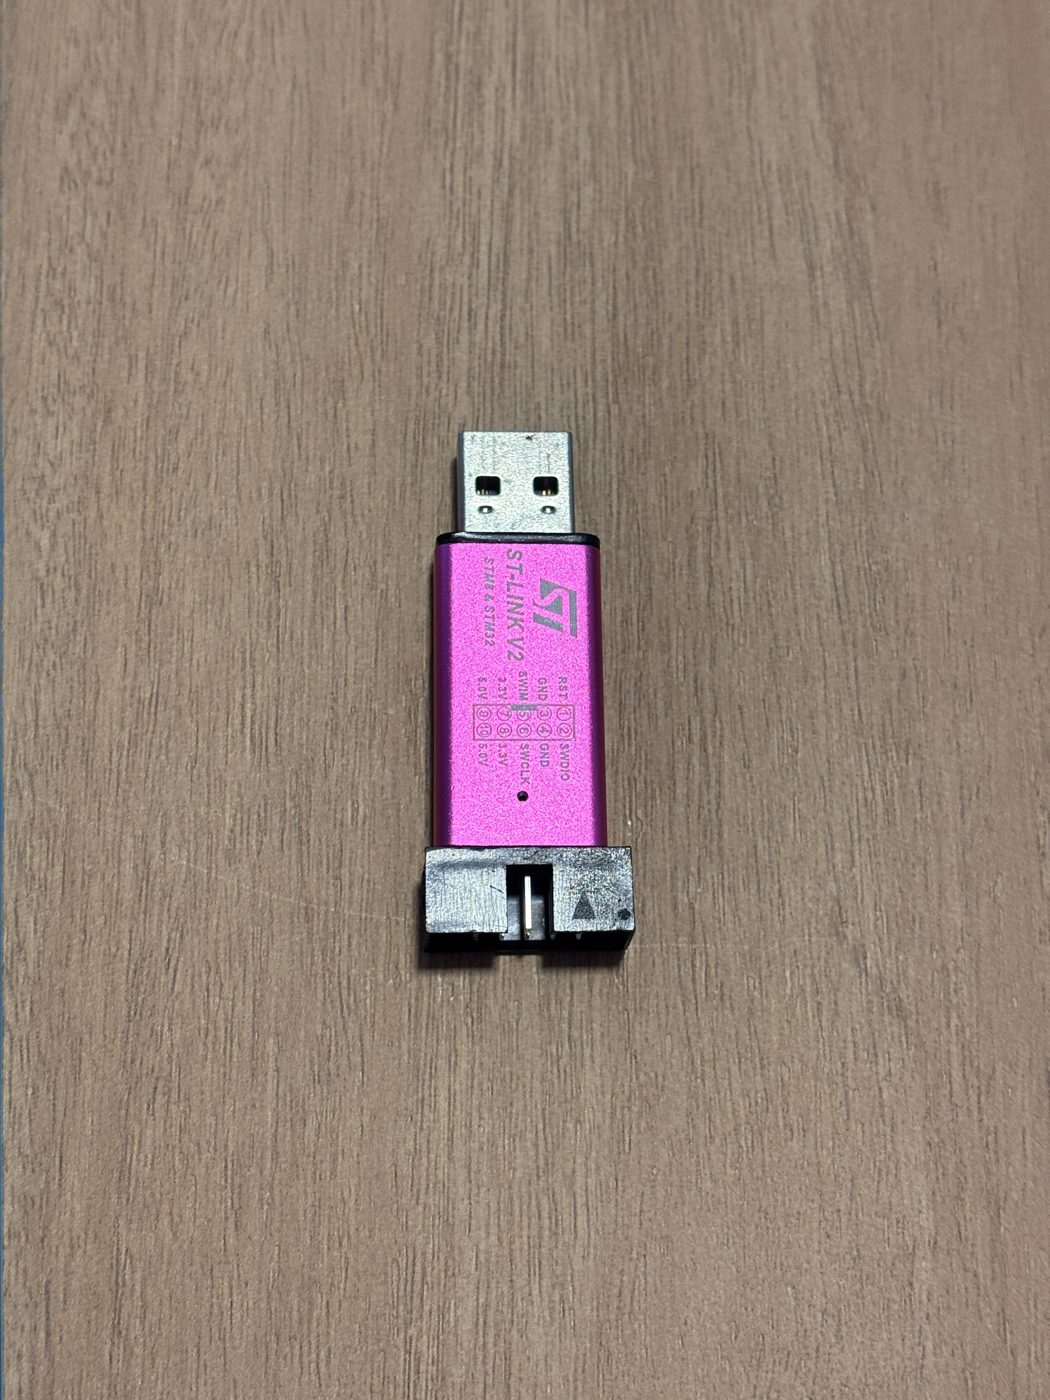
\includegraphics[width=\textwidth]{photos/stlink.jpg}\\(f)\end{minipage}
\fonte{Elaborado pelos autores (2026).}
\end{figure}

\section{ALIMENTAÇÃO}

A fonte de 12~V alimenta o driver diretamente (VM) e, em paralelo, o BEC. A saída de 5~V do BEC passa pela chave deslizante e chega ao pino 5V da Blue Pill; o regulador de 3,3~V da placa alimenta o MPU6050. Todos os terras são comuns. A Figura~\ref{fig:alimentacao} resume o esquema.
\begin{figure}[htbp]
\centering\caption{Distribuição de alimentação.}\label{fig:alimentacao}
\begin{tikzpicture}[node distance=9mm and 11mm,box/.style={draw,align=center,minimum height=10mm,font=\small,text width=2.6cm},arr/.style={-{Latex},thick}]
\node[box] (fonte) {Fonte\\12~V};
\node[box,right=of fonte] (bec) {BEC\\12~V$\to$5~V};
\node[box,right=of bec] (chave) {Chave\\deslizante};
\node[box,right=of chave] (bp) {Blue Pill\\(3,3~V)};
\node[box,below=of bp] (mpu) {MPU6050};
\node[box,below=of bec] (drv) {DRV8871\\(VM = 12~V)};
\node[box,below=of chave] (mot) {Indutor\\+ motor};
\draw[arr] (fonte)--(bec); \draw[arr] (bec)--(chave); \draw[arr] (chave)--(bp);
\draw[arr] (bp)--node[right,font=\scriptsize]{3,3~V}(mpu);
\draw[arr] (fonte.south)|-(drv.west);
\draw[arr] (drv)--(mot);
\end{tikzpicture}
\fonte{Elaborado pelos autores (2026).}
\end{figure}
A chave interrompe somente os 5~V da lógica; o driver continua ligado aos 12~V. Sem os 5~V, o microcontrolador desliga, as entradas do driver ficam sem sinal e o motor para. Assim, a chave faz o papel de liga/desliga do controle, enquanto a fonte de 12~V permanece conectada.

\section{LIGAÇÕES}

\begin{quadro}[htbp]
\centering
\caption{Mapa de interfaces do protótipo.}\label{tab:pinos}
\begin{tabularx}{\textwidth}{|p{1.8cm}|p{2.5cm}|p{3.4cm}|X|}
\hline
\textbf{STM32} & \textbf{Componente} & \textbf{Sinal} & \textbf{Função}\\ \hline
PA9 & DRV8871 & IN2 / TIM1 CH2 & nível alto fixo enquanto a saída é maior que zero (sentido em que a hélice empurra a haste para cima)\\
PA8 & DRV8871 & IN1 / TIM1 CH1 & PWM do motor: com PA9 em nível alto, o motor é acionado enquanto PA8 está baixo e freia quando está alto\\
PB6 & MPU6050 & SCL / I\textsuperscript{2}C1 & relógio do barramento, 400~kHz\\
PB7 & MPU6050 & SDA / I\textsuperscript{2}C1 & dados do barramento\\
PA2 / PA3 & Interface serial & USART2 TX/RX & comandos e telemetria, 115200 8N1 (opcional)\\
PC13 & LED da placa & GPIO & estado: calibrando, rodando, sem sensor\\
PA13 / PA14 & ST-Link & SWDIO / SWCLK & gravação e diagnóstico\\
GND & todos & referência & terra comum\\ \hline
\end{tabularx}
\fonte{Elaborado pelos autores (2026), conforme \texttt{topicos2.ioc}.}
\end{quadro}
A Figura~\ref{fig:esquema} mostra a fiação por pino. O motor fica entre OUT1 e OUT2 do driver, com o indutor em série no fio de OUT1, perto do driver e fora da haste. Não há capacitor externo na entrada VM do driver. Os componentes internos dos módulos MPU6050 e DRV8871, como resistores de \textit{pull-up}, não aparecem no desenho.
\begin{figure}[htbp]
\centering\caption{Diagrama de ligações do protótipo.}\label{fig:esquema}
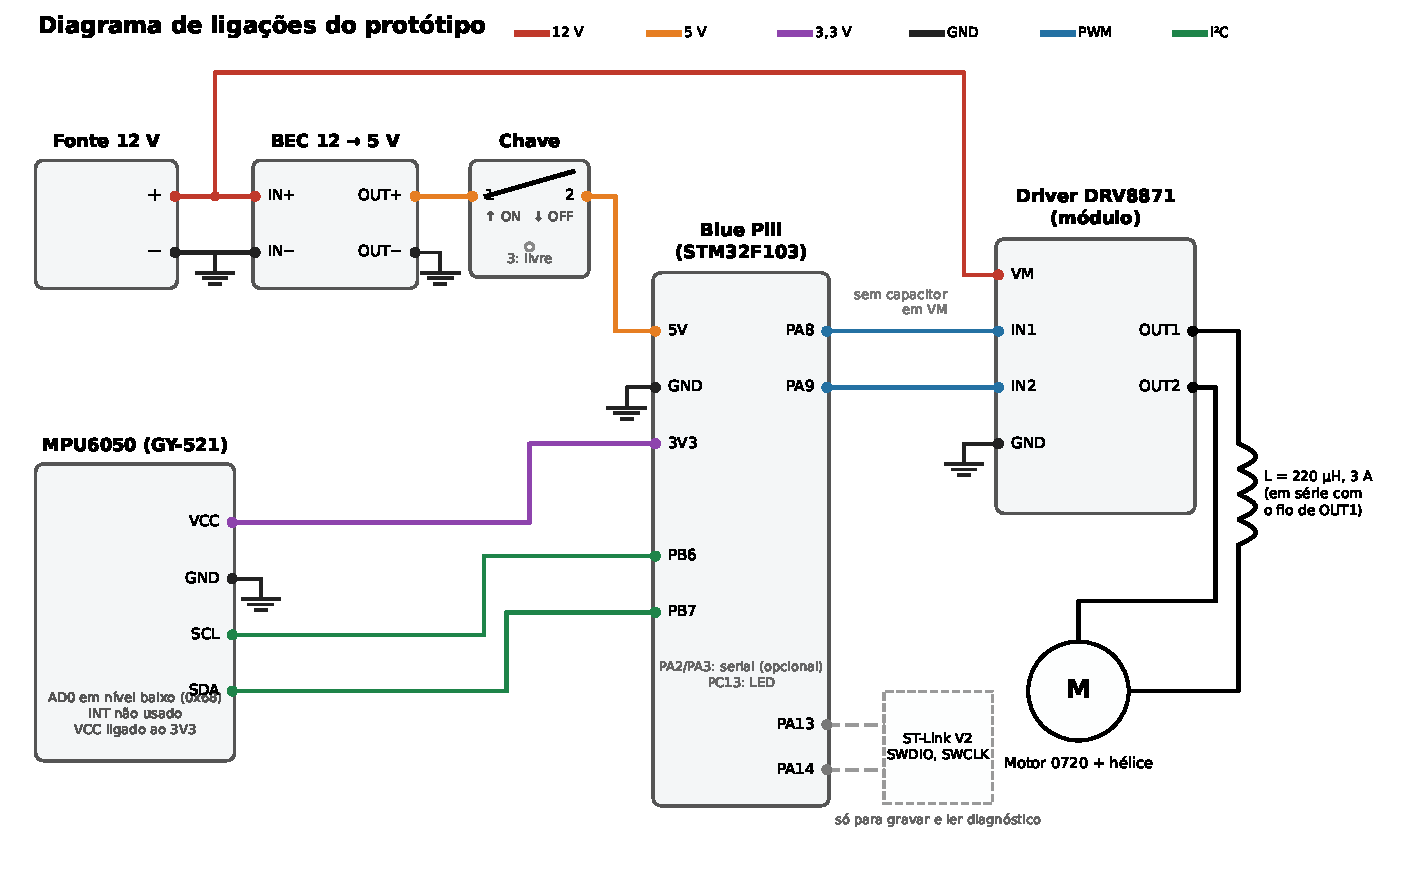
\includegraphics[width=\textwidth]{hardware/esquema_ligacoes.pdf}
\fonte{Elaborado pelos autores (2026), conforme \texttt{topicos2.ioc} e a montagem do protótipo.}
\end{figure}
Um mau contato no cabo do motor chegou a manter a haste parada com saída máxima durante 8~s; por isso todas as ligações foram soldadas.

\section{MONTAGEM MECÂNICA}

A Blue Pill e o driver ficam dentro da caixa fechada. A haste é presa ao suporte por um parafuso com porca travada, que forma o eixo de rotação. O motor com a hélice fica em uma ponta da haste e o MPU6050 na outra, preso com fita dupla face. O sensor está montado de cabeça para baixo e a haste gira em torno do eixo Y dele; o firmware compensa com uma soma de $180^\circ$ ao ângulo (Capítulo~\ref{cap:desenvolvimento}). O sentido de empuxo foi confirmado visualmente na bancada.

\section{PROTÓTIPO FINAL}

A estrutura final tem uma base de madeira, o suporte da haste impresso em 3D, a haste com o motor e a hélice em uma ponta e o MPU6050 na outra, e uma caixa impressa em 3D que abriga a Blue Pill e o driver, com a chave liga/desliga na lateral. As Figuras~\ref{fig:final_cima} a~\ref{fig:final_tras} mostram o protótipo montado.
\begin{figure}[htbp]
\centering\caption{Protótipo final, visto de cima.}\label{fig:final_cima}
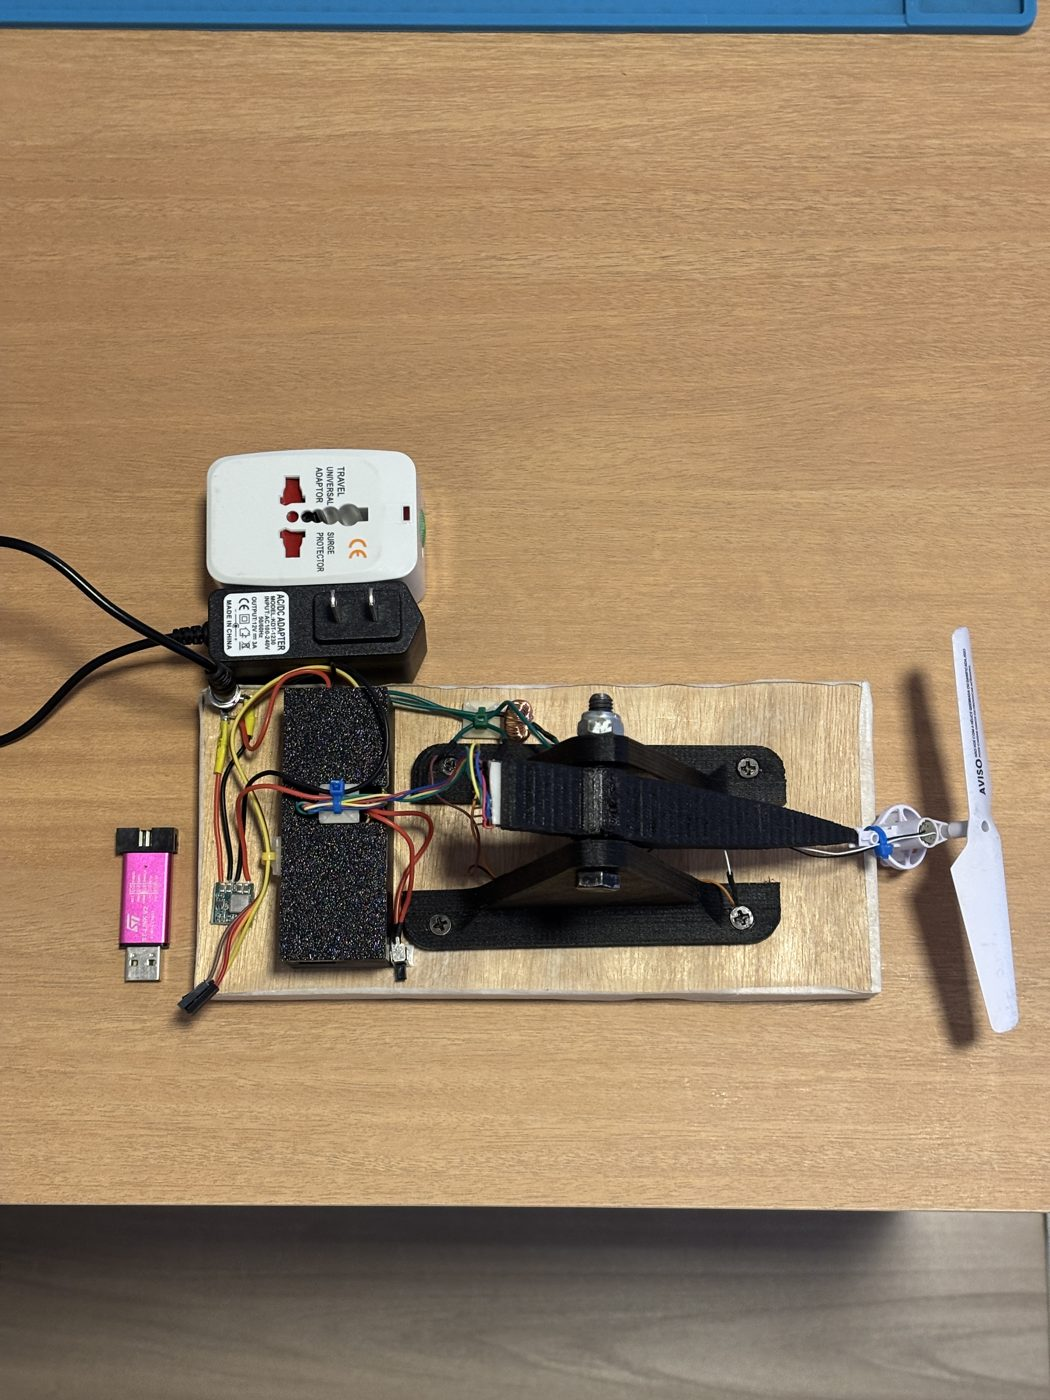
\includegraphics[height=.42\textheight]{photos/final_top.jpg}
\fonte{Elaborado pelos autores (2026).}
\end{figure}
\begin{figure}[htbp]
\centering\caption{Protótipo final: (a) visto de frente e (b) visto de lado.}\label{fig:final_lado}
\begin{minipage}[t]{.48\textwidth}\centering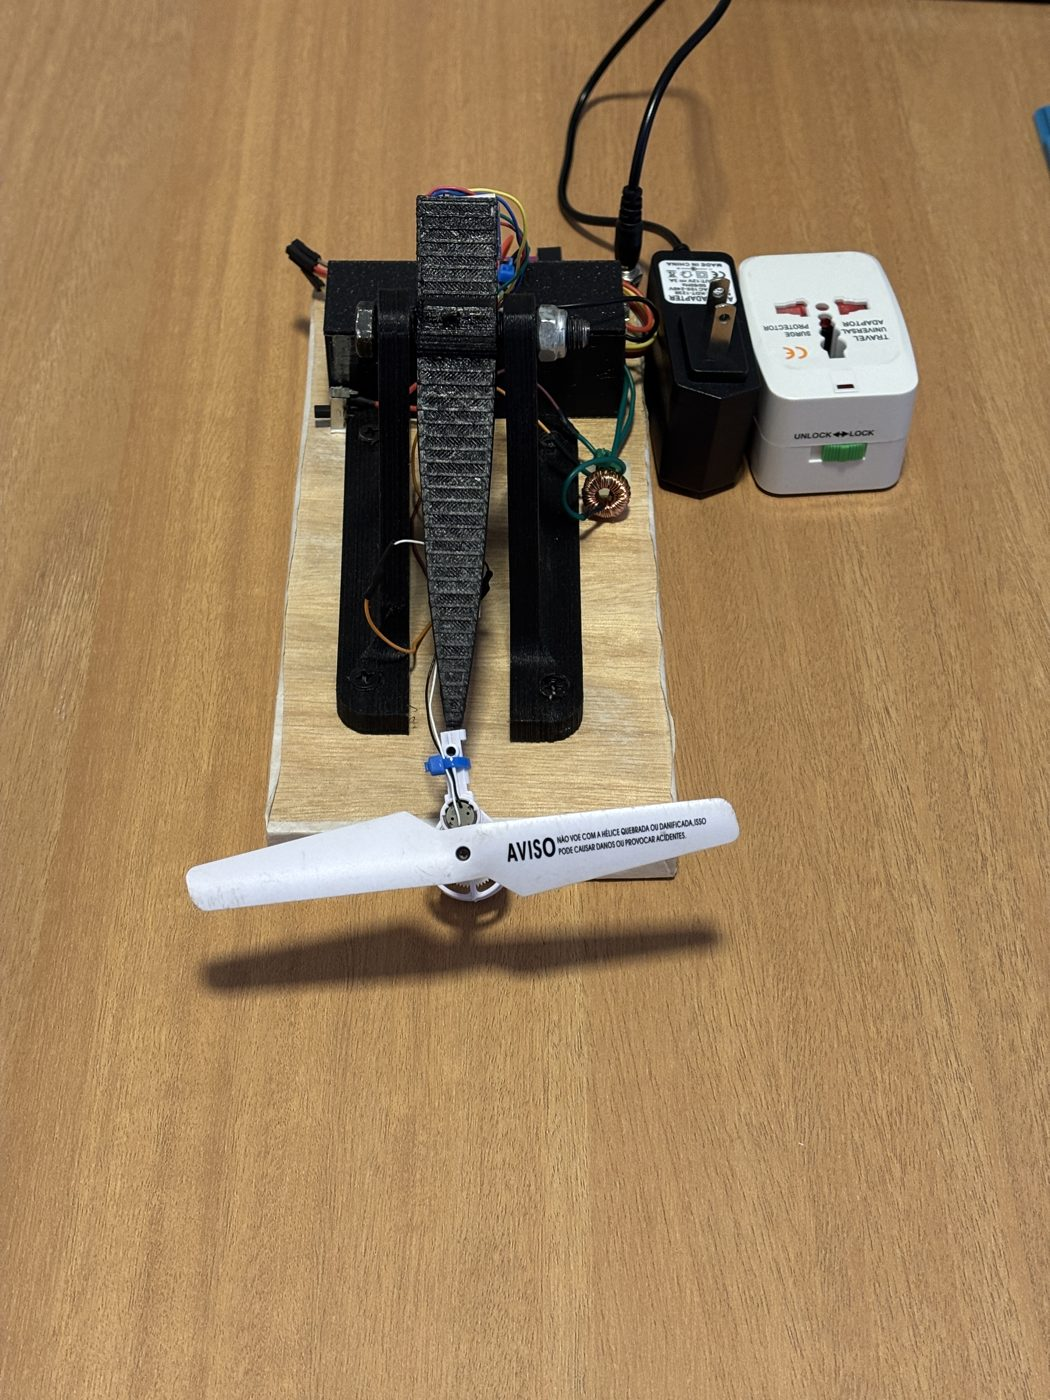
\includegraphics[height=.34\textheight]{photos/final_front.jpg}\\(a)\end{minipage}\hfill
\begin{minipage}[t]{.48\textwidth}\centering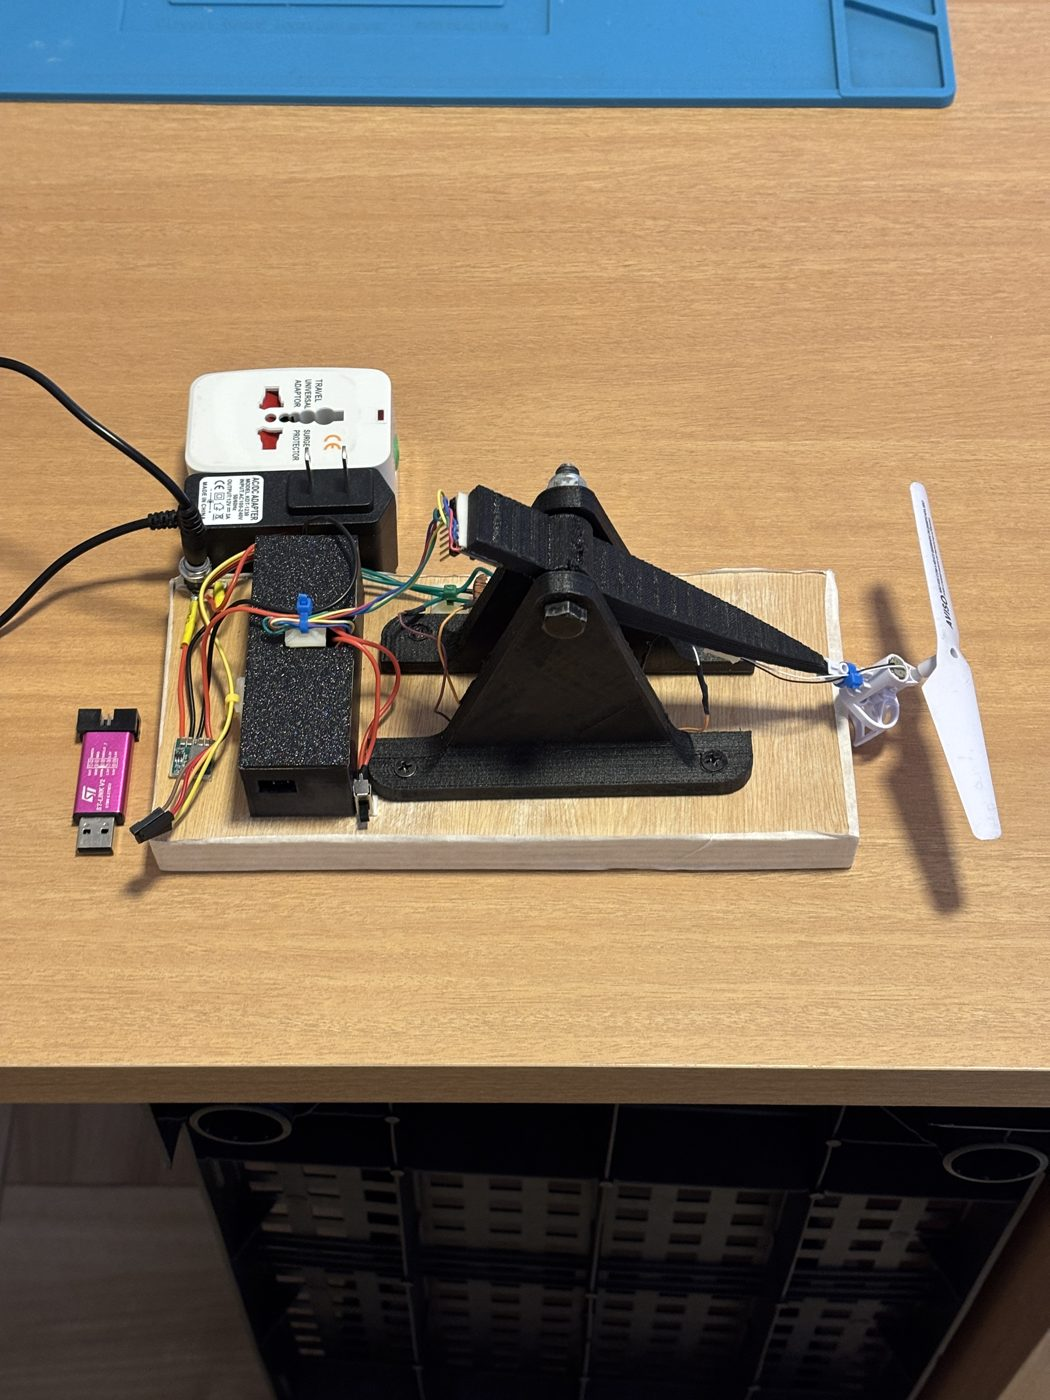
\includegraphics[height=.34\textheight]{photos/final_side_1.jpg}\\(b)\end{minipage}
\fonte{Elaborado pelos autores (2026).}
\end{figure}
\begin{figure}[htbp]
\centering\caption{Protótipo final, visto de trás, com a fonte, o adaptador, a caixa da eletrônica e o ST-Link.}\label{fig:final_tras}
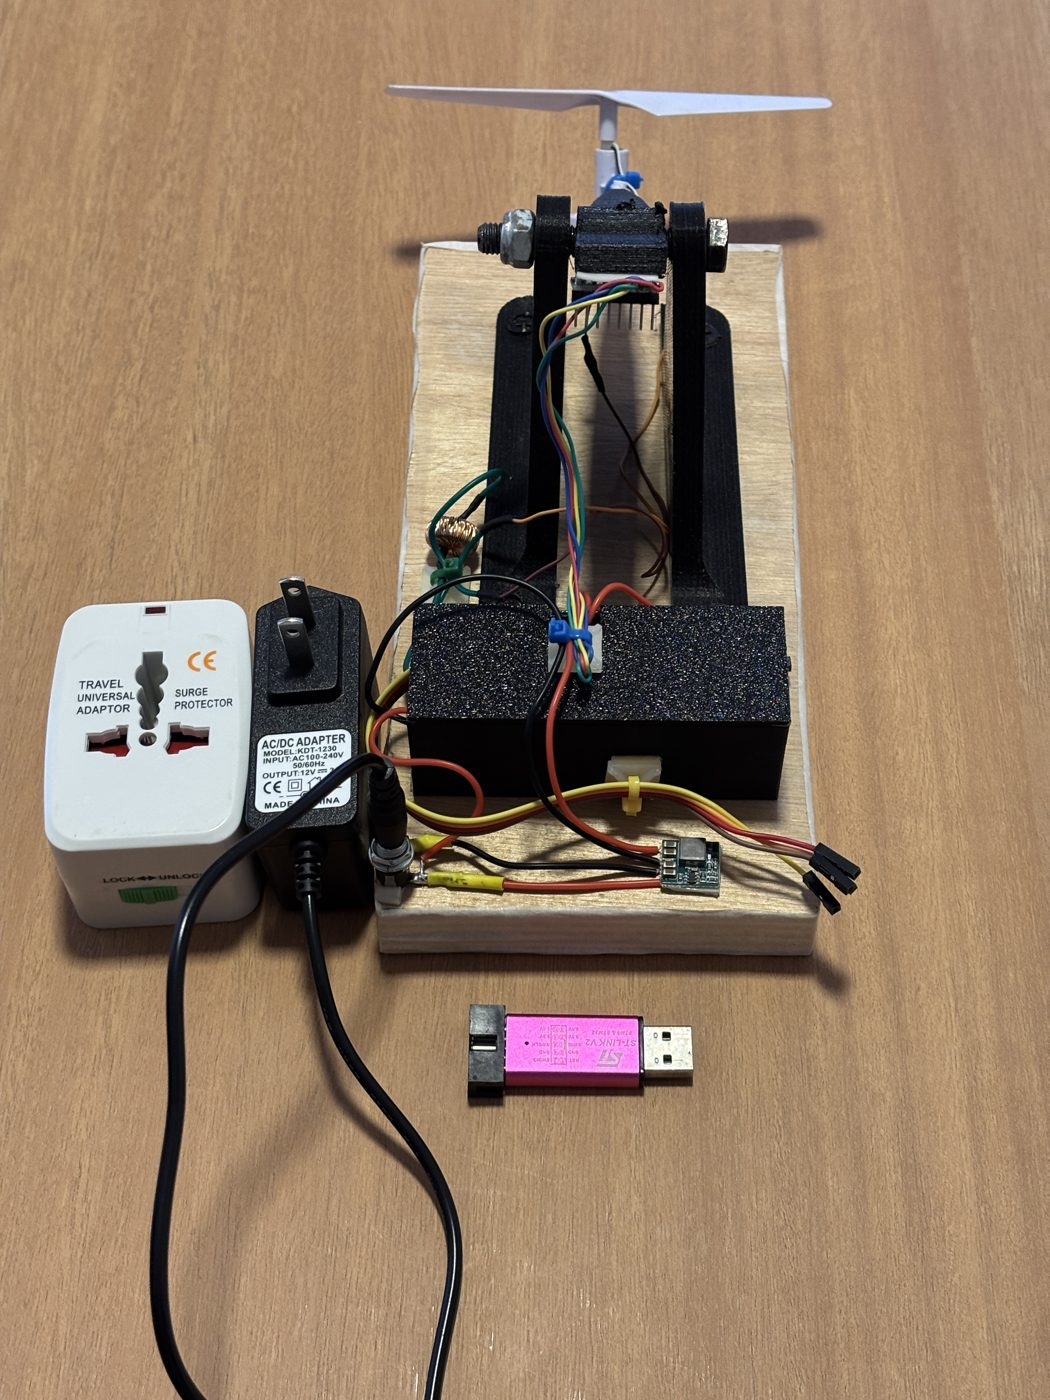
\includegraphics[height=.42\textheight]{photos/final_back.jpg}
\fonte{Elaborado pelos autores (2026).}
\end{figure}
\fotofinal{final_rodando}{Protótipo final com a haste estabilizada, em funcionamento.}{fig:final_rodando}

\section{ESTUDO DA POTÊNCIA DO MOTOR}\label{sec:potencia}

O motor tem tensão nominal de 3,7~V e é alimentado por 12~V através do driver. A tensão média é controlada pelo PWM, limitado a 32\%, o que dá cerca de 3,8~V médios (12~V $\times$ 0,32), próximo do nominal. O DRV8871 desarma por sobrecorrente entre 3,7 e 6,4~A e religa depois de 3~ms, e não funciona abaixo de 6,5~V \cite{drv8871ds}; por isso não dá para alimentá-lo com os 3,7~V do motor. Daí os 12~V com PWM baixo. A Seção~\ref{sec:indutor} mostra o efeito colateral dessa escolha.

\chapter{DESENVOLVIMENTO DO FIRMWARE}\label{cap:desenvolvimento}

Este capítulo reúne o necessário para reproduzir o firmware: ferramentas, configuração do microcontrolador, organização em módulos, tarefas e objetos do FreeRTOS.

\section{FERRAMENTAS E VERSÕES}

\begin{table}[htbp]
\centering\caption{Ambiente de desenvolvimento.}\label{tab:versoes}
\begin{tabularx}{\textwidth}{lX}
\hline\textbf{Item} & \textbf{Versão}\\\hline
IDE / CubeMX & STM32CubeIDE 2.2.0 (projeto gerado com o CubeMX integrado)\\
Pacote do chip & STM32Cube FW\_F1 V1.8.7 (HAL e CMSIS)\\
Compilador & GNU Tools for STM32 14.3.rel1 (\texttt{arm-none-eabi-gcc} 14.3.1), \textit{newlib-nano}\\
FreeRTOS & Kernel V10.3.1, porta ARM\_CM3, \textit{heap\_4}; camada CMSIS-RTOS V2 usada apenas pelo código gerado\\
Gravação e leitura & STM32CubeProgrammer 2.23.0 com ST-Link V2 (SWD)\\
Simulação e análise & Python 3, NumPy, Matplotlib; GCC no computador para \texttt{firmware/tests/sim\_control.c}\\
Verificação de regras & \texttt{firmware/tools/misra\_check.sh} (MISRA C:2012)\\\hline
\end{tabularx}
\fonte{Elaborado pelos autores (2026).}
\end{table}

\section{CONFIGURAÇÃO DO STM32}

\begin{table}[htbp]
\centering\caption{Configuração dos periféricos (\texttt{topicos2.ioc}).}\label{tab:config}
\begin{tabularx}{\textwidth}{lX}
\hline\textbf{Periférico} & \textbf{Configuração}\\\hline
Clock & HSE de 8~MHz, PLL $\times9$: SYSCLK e HCLK de 72~MHz, APB1 de 36~MHz, APB2 de 72~MHz\\
TIM1 (PA8, PA9) & PWM nos canais 1 e 2; o CubeMX configura 20~kHz e \texttt{Motor\_Init} recalcula para 100~kHz (prescaler 0, ARR 719)\\
TIM2 & Prescaler 7199 e período 49: estouro a 200~Hz (5~ms), com interrupção; libera o semáforo de controle\\
I2C1 (PB6, PB7) & Modo rápido, 400~kHz\\
USART2 (PA2, PA3) & 115200 bit/s, 8N1; recepção por interrupção\\
Base de tempo da HAL & TIM4 (o SysTick fica com o FreeRTOS)\\
FreeRTOS & \textit{tick} de 1~kHz, preempção ligada, \textit{heap} de 8192~bytes, 56 níveis de prioridade, \textit{mutexes} e semáforos contadores ligados\\
NVIC & Grupo de prioridades 4 (4 bits de preempção); TIM2 e USART2 em prioridade 5, igual ao limite \texttt{configMAX\_SYSCALL\_INTERRUPT\_PRIORITY}; PendSV e SysTick em 15\\\hline
\end{tabularx}
\fonte{Elaborado pelos autores (2026).}
\end{table}
O MPU6050 é configurado por \texttt{Mpu\_Init}: relógio pelo PLL do giroscópio, filtro digital de 44~Hz, taxa de saída de 200~Hz, giroscópio de $\pm1000^\circ$/s e acelerômetro de $\pm16$~g. As escalas largas evitam saturar o sensor na queda da haste ($>500^\circ$/s) e na vibração da hélice.

\section{ORGANIZAÇÃO EM MÓDULOS}

O código escrito pelo grupo fica em \texttt{firmware/Modules/}, separado do código gerado pelo CubeMX (\texttt{firmware/Core/}). Cada módulo tem uma responsabilidade; o módulo de controle não depende de hardware nem de RTOS, o que permite executá-lo no computador.
\begin{table}[htbp]
\centering\caption{Módulos do firmware.}\label{tab:modulos}
\begin{tabularx}{\textwidth}{lX}
\hline\textbf{Módulo} & \textbf{Conteúdo}\\\hline
\texttt{app/} & \texttt{app\_config.h}: todos os ajustes em um só lugar; \texttt{app.c}: tarefa de controle, semáforo, \textit{mutex} de dados e acesso aos dados compartilhados\\
\texttt{sensor/} & \texttt{mpu6050.c}: leitura por I\textsuperscript{2}C e conversão de escalas; \texttt{angle\_filter.c}: filtro complementar\\
\texttt{control/} & \texttt{pid.c}: PID com derivada na medida e anti-\textit{windup}; \texttt{control.c}: filtro da derivada e rampa da saída\\
\texttt{motor/} & \texttt{motor.c}: PWM do DRV8871 (frequência, modo de freio, limite)\\
\texttt{serial/} & \texttt{serial.c}: comandos, telemetria, LED, tarefas de comando e telemetria, fila e \textit{mutex} da UART\\
\texttt{debug/} & \texttt{debug.c}: contadores e registro circular na RAM, lidos pelo ST-Link sem serial\\\hline
\end{tabularx}
\fonte{Elaborado pelos autores (2026).}
\end{table}

Todo o código escrito pelo grupo segue o mesmo padrão. As funções públicas são documentadas com Doxygen, em português, e os trechos feitos à mão (PID, filtro, registradores do MPU6050, PWM do DRV8871) citam a fonte consultada. Os nomes indicam o módulo, o tipo e a unidade, como em \texttt{Motor\_Set}, \texttt{Pid\_t} e \texttt{angle\_deg}. Os módulos foram conferidos com as regras do MISRA C:2012; os desvios são todos de regras \textit{advisory}: uso direto de \texttt{float} (Dir.~4.6), conversões de endereço feitas pelas macros da HAL (Reg.~11.4) e funções globais exigidas pela HAL e pelo CubeMX (Reg.~8.7).

Todos os ajustes do projeto ficam em um único arquivo, \texttt{app\_config.h}. As Tabelas~\ref{tab:parametros_fw}, \ref{tab:parametros_motor} e~\ref{tab:parametros_ctrl} explicam cada valor e o motivo da escolha.
\begin{table}[H]
\centering\caption{Parâmetros de amostragem e sensor (\texttt{app\_config.h}).}\label{tab:parametros_fw}
\begin{tabularx}{\textwidth}{>{\raggedright\arraybackslash}p{3.7cm}>{\raggedright\arraybackslash}p{2.3cm}X}
\hline\textbf{Parâmetro} & \textbf{Valor} & \textbf{Significado e motivo}\\\hline
\texttt{CTRL\_PERIOD\_S} & 0,005 s & Período do laço de controle (200~Hz), gerado pelo TIM2. É cerca de doze vezes menor que o atraso do empuxo.\\
\texttt{IMU\_AXIS\_X} & 0 & A haste gira em torno do eixo Y do sensor: o ângulo vem de \texttt{atan2(-ax, az)} e a velocidade, do giroscópio Y.\\
\texttt{ANGLE\_OFFSET\_DEG} & 180$^\circ$ & Soma ao ângulo medido para compensar o sensor montado de cabeça para baixo, de modo que $0^\circ$ seja a horizontal.\\
\texttt{COMP\_TAU\_S} & 2,0 s & Constante do filtro complementar com o motor parado: em escalas de tempo menores que ela, vale o giroscópio; em maiores, o acelerômetro.\\
\texttt{COMP\_TAU\_FLIGHT\_S} & 30 s & Constante do filtro com o motor ligado. Em voo o acelerômetro é ruidoso, mas não deriva; uma correção muito lenta segura a deriva do giroscópio sem deixar o ruído passar.\\
\texttt{ACC\_FLIGHT\_GATE\_DEG} & 25$^\circ$ & Em voo, descarta a leitura do acelerômetro que difira da estimativa por mais que isso (as amostras de $-48^\circ$ a $+46^\circ$ vistas em voo).\\
\hline
\end{tabularx}
\fonte{Elaborado pelos autores (2026).}
\end{table}

\begin{table}[H]
\centering\caption{Parâmetros do motor (\texttt{app\_config.h}).}\label{tab:parametros_motor}
\begin{tabularx}{\textwidth}{>{\raggedright\arraybackslash}p{3.7cm}>{\raggedright\arraybackslash}p{2.3cm}X}
\hline\textbf{Parâmetro} & \textbf{Valor} & \textbf{Significado e motivo}\\\hline
\texttt{MOTOR\_SIGN} & $-1$ & Escolhe IN2 (PA9) como a entrada que aciona o motor, o sentido em que a hélice empurra a haste para cima. O motor nunca gira ao contrário.\\
\texttt{MOTOR\_PWM\_HZ} & 100~kHz & Frequência do PWM. É alta para que a corrente do motor, que tem indutância muito baixa, fique lisa. Em 1 e 20~kHz o driver desarmou; em 200~kHz a haste não equilibrou.\\
\texttt{MOTOR\_SLOW\_DECAY} & 1 & Entre os pulsos, o motor é freado em vez de solto. Com o indutor, a corrente fica lisa e a tensão média no motor é a saída em porcentagem vezes 12~V.\\
\texttt{OUT\_LIMIT\_PCT} & 32\% & Teto da saída. Com 12~V equivale a cerca de 3,8~V médios, perto dos 3,7~V nominais; acima disso o motor esquentou.\\
\texttt{MOTOR\_IDLE\_PCT} & 10\% & Saída mínima com o controle ativo: a hélice nunca para, o que evita o tempo de partida a cada correção.\\
\texttt{OUT\_SLEW\_PCT\_S} & 300\%/s & Variação máxima da saída (1,5 ponto por ciclo). Protege o driver de degraus de corrente; desligar o motor é sempre imediato.\\
\hline
\end{tabularx}
\fonte{Elaborado pelos autores (2026).}
\end{table}

\begin{table}[H]
\centering\caption{Parâmetros do controle e da partida (\texttt{app\_config.h}).}\label{tab:parametros_ctrl}
\begin{tabularx}{\textwidth}{>{\raggedright\arraybackslash}p{3.7cm}>{\raggedright\arraybackslash}p{2.3cm}X}
\hline\textbf{Parâmetro} & \textbf{Valor} & \textbf{Significado e motivo}\\\hline
\texttt{KP\_DEFAULT} & 0,06 \%/$^\circ$ & Ganho proporcional: cada grau de erro soma 0,06 ponto percentual de PWM.\\
\texttt{KI\_DEFAULT} & 0,08 \%/($^\circ$\,s) & Ganho integral: corrige o erro que persiste e sustenta a haste no PWM de pairar. Era 0,05 no projeto; subiu para 0,08 no refino (Capítulo~\ref{cap:refino}).\\
\texttt{KD\_DEFAULT} & 0,04 \%/($^\circ$/s) & Ganho derivativo: freia o movimento usando a velocidade do giroscópio, o que dá amortecimento.\\
\texttt{RATE\_FILTER\_TAU\_S} & 5 ms & Filtro passa-baixas da velocidade usada no termo derivativo, para que a vibração da hélice não vire pulsos na saída. Valores maiores reduzem a margem de fase.\\
\texttt{OUT\_HOVER\_PCT} & 16\% & Valor inicial do integrador, um pouco abaixo do PWM necessário para pairar (cerca de 20\%). Sem ele, a haste levaria mais de 8~s para sair do repouso; começar abaixo evita que ela passe do alvo.\\
\texttt{SETPOINT\_DEFAULT\_DEG} & 0,7$^\circ$ & Ângulo-alvo da haste; pode ser alterado pela serial entre $\pm60^\circ$.\\
\texttt{AUTO\_ARM} & 1 & O motor liga sozinho ao fim da calibração de 2~s, sem comando da serial.\\
\texttt{ANGLE\_CUTOFF\_HI\_DEG} / \texttt{LO} & $+60^\circ$ / $-90^\circ$ & Corte por ângulo: fora dessa faixa o motor é desligado e só volta com o comando de armar ou com o reset.\\\hline
\end{tabularx}
\fonte{Elaborado pelos autores (2026).}
\end{table}

\section{TAREFAS E OBJETOS DO FREERTOS}

A aplicação tem três tarefas além da ociosa e da de temporizadores do núcleo. A tarefa de controle executa em sequência sensor, filtro, PID e motor, de modo que a amostra lida é usada no mesmo ciclo e nenhuma etapa atrasa a outra.
\begin{table}[htbp]
\centering\caption{Tarefas do sistema.}\label{tab:tarefas}
\begin{tabularx}{\textwidth}{llllX}
\hline\textbf{Tarefa} & \textbf{Prio.} & \textbf{Pilha (palavras)} & \textbf{Período} & \textbf{Função}\\\hline
\texttt{control} & 3 & 384 & 5 ms (semáforo) & lê o MPU6050, filtra, calcula o PID e atualiza o PWM\\
\texttt{cmd} & 2 & 192 & por evento (fila) & monta linhas de comando da serial e as aplica\\
\texttt{telem} & 1 & 192 & 50 ms (\texttt{vTaskDelayUntil}) & envia ângulo, alvo e saída; pisca o LED\\
Ociosa e temporizadores & 0 e 2 & 128 e 256 & --- & núcleo do FreeRTOS (a tarefa \texttt{defaultTask} do CubeMX se apaga ao iniciar)\\\hline
\end{tabularx}
\fonte{Elaborado pelos autores (2026), conforme \texttt{app.c} e \texttt{serial.c}.}
\end{table}

\begin{table}[htbp]
\centering\caption{Objetos de sincronização.}\label{tab:objetos}
\begin{tabularx}{\textwidth}{llX}
\hline\textbf{Objeto} & \textbf{Tipo} & \textbf{Uso}\\\hline
\texttt{s\_tickSem} & semáforo binário & a ISR do TIM2 (\texttt{xSemaphoreGiveFromISR}) acorda a tarefa de controle a cada 5~ms\\
\texttt{s\_dataMutex} & \textit{mutex} & protege ganhos, alvo e telemetria entre \texttt{control}, \texttt{cmd} e \texttt{telem}\\
\texttt{s\_uartMutex} & \textit{mutex} & uma tarefa por vez transmite pela USART2\\
\texttt{s\_rxQueue} & fila de 32 bytes & ISR de recepção $\to$ \texttt{cmd}\\\hline
\end{tabularx}
\fonte{Elaborado pelos autores (2026).}
\end{table}

\begin{figure}[htbp]
\centering\caption{Fluxo entre interrupções, objetos do FreeRTOS e tarefas.}\label{fig:fluxogeral}
\begin{tikzpicture}[node distance=10mm and 12mm,box/.style={draw,align=center,text width=3.1cm,minimum height=11mm,font=\small},obj/.style={draw,rounded corners,align=center,font=\footnotesize,minimum height=7mm,fill=gray!15},arr/.style={-{Latex},thick}]
\node[box] (tim) {TIM2 (ISR)\\200 Hz};
\node[obj,right=of tim] (sem) {semáforo\\\texttt{s\_tickSem}};
\node[box,right=of sem] (ctl) {\texttt{control} (prio. 3)\\MPU6050, filtro, PID, PWM};
\node[box,below=14mm of ctl] (mtx) {\texttt{s\_dataMutex}: ganhos, alvo, telemetria};
\node[box,below=14mm of tim] (rx) {USART2 RX (ISR)};
\node[obj,right=of rx] (q) {fila\\\texttt{s\_rxQueue}};
\node[box,below=12mm of q] (cmd) {\texttt{cmd} (prio. 2)};
\node[box,right=of cmd] (tel) {\texttt{telem} (prio. 1)\\20 Hz + LED};
\draw[arr] (tim)--(sem); \draw[arr] (sem)--(ctl);
\draw[arr] (rx)--(q); \draw[arr] (q)--(cmd);
\draw[arr] (ctl)--(mtx); \draw[arr] (cmd.east)--(tel.west) node[midway,above,font=\scriptsize]{};
\draw[arr] (cmd.north east)|-(mtx.west);
\draw[arr] (tel.north)--(mtx.south);
\end{tikzpicture}
\fonte{Elaborado pelos autores (2026).}
\end{figure}

\subsection{Por que uma única tarefa para a malha crítica}

As tarefas foram divididas por ritmo e criticidade, e não por função do código. Leitura do sensor, filtro, PID e atualização do motor ocorrem todos a cada 5~ms, em sequência, e cada etapa usa o resultado da anterior no mesmo ciclo. Como o STM32F103 tem um único núcleo, dividir essa cadeia em várias tarefas não traria paralelismo e acrescentaria filas, trocas de contexto e o risco de o PID usar uma amostra de ciclo anterior. O critério de divisão por período, prioridade e bloqueio é o recomendado na literatura de tempo real \cite{buttazzo2011,burns2009,barry2016}. Aqui há um sensor e uma taxa; controladores de voo maiores separam estimador e controle por terem vários sensores em taxas diferentes.

A malha de controle, sozinha, também poderia ser feita sem RTOS, como na versão anterior em Arduino. O que o FreeRTOS acrescenta está em volta dela:
\begin{itemize}
 \item a tarefa \texttt{control}, de prioridade 3, interrompe as tarefas lentas (comandos e telemetria pela serial, que envia por espera ativa) sem nenhuma lógica extra de interrupção;
 \item a tarefa dorme no semáforo e acorda a cada 5~ms; o limite de espera de 20~ms também serve para detectar a falha do sensor;
 \item o \textit{mutex} com herança de prioridade protege os dados que as três tarefas compartilham;
 \item funções novas, como um \textit{watchdog}, entram como tarefas novas, sem reescrever o laço principal.
\end{itemize}
O FreeRTOS não deixa o controle mais rápido nem garante o prazo sozinho; se o prazo é cumprido, quem mostra é a análise temporal (Seção~\ref{sec:temporal}). Duas melhorias possíveis não foram implementadas: ler o sensor por DMA, em vez de espera ativa de cerca de 0,4 a 0,6~ms, e disparar o ciclo pelo pino de dado pronto do MPU6050, em vez do TIM2, para fixar a idade da amostra.

\subsection{Ciclo de controle}

A cada estouro do TIM2, a interrupção só libera o semáforo (processamento diferido); todo o trabalho acontece na tarefa. A tarefa então: (i) espera o semáforo por até 20~ms; (ii) lê 14~bytes do MPU6050 por I\textsuperscript{2}C a 400~kHz; (iii) atualiza o ângulo pelo filtro complementar (rápido com o motor parado, lento e com janela de rejeição em voo) e confere o corte por ângulo; (iv) copia os parâmetros sob o \textit{mutex}; (v) executa o PID e a rampa de saída; (vi) escreve o PWM; (vii) grava o registro de diagnóstico e a telemetria. A tarefa de telemetria tem prioridade menor que a de controle: se o envio pela serial demorar, ele é interrompido e a leitura do sensor e o cálculo do motor continuam no prazo. Se 10 ciclos seguidos (50~ms) falharem, a tarefa desliga o motor e tenta reiniciar o sensor (e o barramento I\textsuperscript{2}C, se necessário), voltando a controlar quando ele responde; o integrador recomeça em 16\%.

\subsection{Partida e proteção}

Após o reset, o LED fica aceso e a tarefa mede, durante 2~s com a haste parada (400 amostras), o viés do giroscópio e o ângulo inicial pelo acelerômetro. Em seguida o controle arma automaticamente (\texttt{AUTO\_ARM}). Há duas proteções: o motor desliga se o sensor ficar 50~ms sem responder ou se o ângulo sair da faixa de $-90^\circ$ a $+60^\circ$; neste segundo caso, ele só volta com o comando de armar ou com o reset. O corte foi acrescentado depois de a haste dar uma volta completa em 02/11/2026 (Seção~\ref{sec:deriva}). O motor também pode ser desligado por comando serial ou pelo ST-Link.

\subsection{Diagnóstico sem serial}

Como não havia conversor USB-serial, o firmware guarda na RAM os contadores de falhas, a folga de pilha e de \textit{heap}, os tempos de cada ciclo (medidos pelo contador de ciclos do DWT) e um registro circular de 320 amostras com ângulo, velocidade, aceleração em X e Z e saída. O \textit{script} \texttt{firmware/tools/dbg\_read.py} lê tudo isso pelo ST-Link sem parar o processador. Esse mesmo registro fornece os dados da Seção~\ref{sec:ruido}.

\section{USO DE MEMÓRIA}

Segundo \texttt{arm-none-eabi-size}, o executável tem 42\,516~bytes de código, 116 de dados inicializados e 17\,364 de dados não inicializados, ou seja, cerca de 42~kB de Flash e 17~kB dos 20~kB de SRAM, dos quais 8~kB são o \textit{heap} do FreeRTOS e cerca de 3,3~kB o registro de diagnóstico. As tarefas ociosa e de temporizadores usam memória estática alocada pela camada CMSIS-RTOS, fora do \textit{heap}; este guarda as pilhas das três tarefas da aplicação (1\,536, 768 e 768~bytes), seus blocos de controle e os objetos de sincronização. Lido pelo ST-Link, o \textit{heap} tinha 4\,168~bytes livres em operação, com menor folga já vista de 3\,472~bytes (o pico ocorre na partida, enquanto a tarefa padrão do CubeMX ainda existe). A estimativa por configuração indicava 2~kB livres; a medida mostra que ela foi conservadora.

Com a haste pairando, a folga mínima de pilha foi de 289 palavras na tarefa \texttt{control} (de 384), 139 na \texttt{cmd} (de 192) e 127 na \texttt{telem} (de 192). O uso máximo ficou entre 25\% e 34\% de cada pilha.

\section{ANÁLISE TEMPORAL}\label{sec:temporal}

O período de 5~ms é o prazo de cada atualização, e vem do TIM2 (cristal de 8~MHz, PLL $\times9$, prescaler 7199 e período 49). Para medir os tempos, o firmware usa o contador de ciclos do DWT do Cortex-M3 (72~MHz, 13,9~ns por ciclo): a interrupção do TIM2 registra o instante em que ocorre; a tarefa \texttt{control} registra o instante em que acorda e o instante em que o PWM é escrito. As medidas vão para a RAM e são lidas pelo ST-Link, sem parar o processador, junto com dois histogramas (latência em caixas de 50~$\mu$s e intervalo entre interrupções em caixas de 1~$\mu$s). A Tabela~\ref{tab:orcamento} compara as estimativas de projeto, feitas antes da medição a partir do datasheet e da ordem de grandeza em ciclos do Cortex-M3 sem unidade de ponto flutuante, com os valores medidos na bancada em 34\,870 ciclos (174~s), com a haste pairando e a telemetria ativa. Uma versão anterior do firmware, sem os histogramas, foi medida por 153\,773 ciclos (768~s, cerca de 12,8~min) com resultados equivalentes: nenhum tick perdido, nenhum atraso de prazo, latência máxima de 560,3~$\mu$s e intervalo entre interrupções de 4\,998,3 a 5\,009,5~$\mu$s.
\begin{table}[htbp]
\centering\caption{Tempos de uma atualização: estimativa e medição.}\label{tab:orcamento}
\begin{tabularx}{\textwidth}{Xrr}
\hline\textbf{Grandeza} & \textbf{Estimativa} & \textbf{Medido}\\\hline
Intervalo entre interrupções do TIM2 & 5\,000~$\mu$s & 4\,998,3 a 5\,009,5~$\mu$s\\
Interrupção até a tarefa acordar & 5 a 20~$\mu$s & máx. 30,4~$\mu$s\\
Tarefa acordada até o PWM escrito (I\textsuperscript{2}C, filtro, PID, PWM) & 540 a 980~$\mu$s & máx. 549,3~$\mu$s\\
Interrupção até o PWM escrito & 550 a 1\,000~$\mu$s & máx. 579,5~$\mu$s; média 557,6~$\mu$s\\
Utilização do período (máximo) & 11\% a 20\% & 11,6\%\\
Interrupções contadas, tarefas acordadas e ticks perdidos & --- & 34\,870, 34\,870 e 0\\
Ciclos com latência acima de 5~ms & --- & 0\\\hline
\end{tabularx}
\fonte{Elaborado pelos autores (2026). Medições da bancada em 02/11/2026.}
\end{table}
A distribuição dos tempos é estreita (Figura~\ref{fig:histo_tempo}): 99,82\% das latências ficaram entre 550 e 600~$\mu$s, e o restante entre 500 e 550~$\mu$s.
\begin{figure}[htbp]
\centering\caption{Histogramas da latência e do intervalo entre interrupções (escala vertical logarítmica).}\label{fig:histo_tempo}
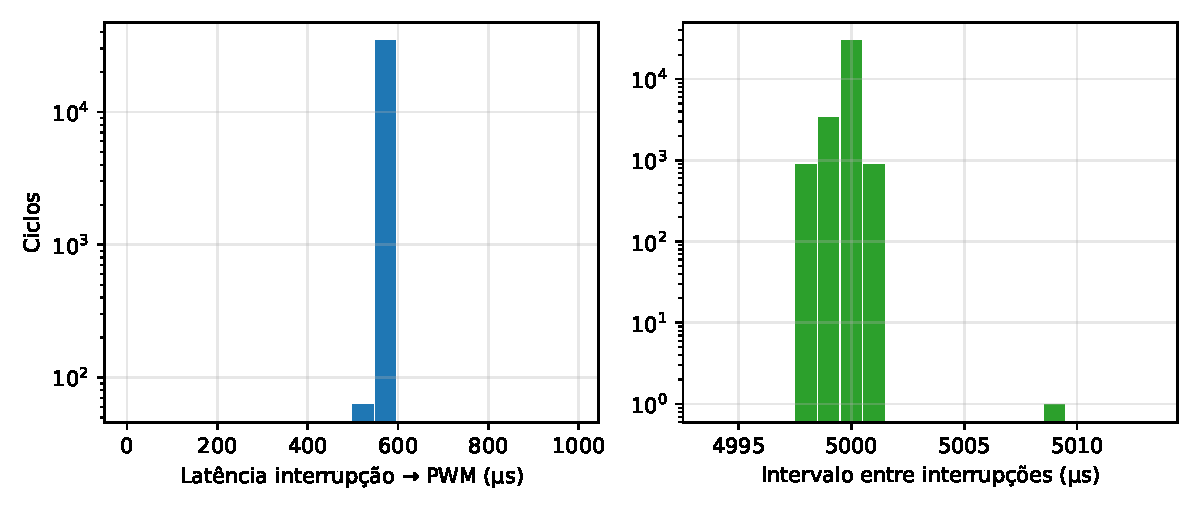
\includegraphics[width=.95\textwidth]{results/histogramas_tempo.pdf}
\fonte{Elaborado pelos autores (2026), dados da bancada.}
\end{figure}
O atraso total entre a interrupção e o PWM ficou em no máximo 580~$\mu$s, ou 11,6\% do prazo, dentro da faixa estimada (no limite inferior dela). A medida é dominada pela leitura I\textsuperscript{2}C de 14~bytes, feita por espera ativa, que ocupa cerca de 0,5~ms. O intervalo entre interrupções ficou entre 4\,998 e 5\,002~$\mu$s em todos os ciclos menos um, que chegou a 5\,009,5~$\mu$s: um \textit{jitter} de no máximo 11,2~$\mu$s, causado por outras interrupções curtas (SysTick, TIM4 da HAL, USART2). A tarefa levou no máximo 30,4~$\mu$s para acordar. A tarefa \texttt{control}, de maior prioridade, só pode ser atrasada por essas interrupções e por regiões críticas do núcleo; o \textit{mutex} \texttt{s\_dataMutex} é mantido apenas durante a cópia de uma estrutura de poucos bytes e conta com herança de prioridade. A transmissão pela UART, por espera ativa na tarefa \texttt{telem}, de prioridade menor, é interrompida pela tarefa \texttt{control}.

Há ainda o atraso dos dados, que independe do RTOS: o filtro digital do MPU6050 em 44~Hz atrasa o sinal em cerca de 5~ms \cite{mpu6050rm}, e como a amostragem do sensor (200~Hz) não é sincronizada com o TIM2, a amostra lida tem idade de 0 a 5~ms. Somados, esses efeitos têm a mesma ordem dos 9~ms de atraso puro identificados na planta (Tabela~\ref{tab:parametros}).

O maior valor observado é evidência experimental da bancada, mas não prova o pior caso de todas as execuções possíveis \cite{buttazzo2011}. A medição foi feita com a telemetria ativa; não foi repetida com ela desligada.

\chapter{DIFICULDADES ENCONTRADAS E SOLUÇÕES}\label{cap:dificuldades}

\section{AQUECIMENTO DO MOTOR E O INDUTOR}\label{sec:indutor}

O motor \textit{coreless} 0720 aquecia a ponto de não se poder tocá-lo. Os 12~V do driver sobre um motor de 3,7~V forçam um PWM de razão cíclica baixa, e esse motor tem indutância muito pequena (estimada em cerca de 7~$\mu$H, constante de tempo elétrica de poucos microssegundos, extrapolada de dados da maxon para motores \textit{coreless} de 8~mm \cite{maxonchoke}). O período de 10~$\mu$s do PWM a 100~kHz não alisa a corrente: ela acompanha cada pulso de 12~V, com picos de cerca de 2~A, e como o calor depende da corrente eficaz, e não da média, o motor dissipava cerca de 1,5~W contra 0,3~W em corrente contínua. Em 20~kHz e 1~kHz o modelo prevê corrente por pulso acima de 4~A, e o DRV8871 desarmava (religação em 3~ms), o que se ouvia como um zumbido agudo seguido do motor parando.

Duas observações apoiam essa explicação: o motor ligado direto em duas pilhas AA (cerca de 3~V, sem driver) não esquentou; e, em 200~kHz, a haste não equilibrou, provavelmente porque os pulsos ficam curtos demais para o driver, cujo pulso mínimo é de 800~ns \cite{drv8871ds}. Os valores de corrente vêm do cálculo em \texttt{firmware/tools/pwm\_heat.py}; a corrente de pico não foi medida.

A solução foi um indutor de potência em série com o motor. Antes, um capacitor em paralelo com o motor foi testado e não resolveu. O cálculo indicava 100~$\mu$H, e qualquer valor de 47 a 220~$\mu$H serve; foi instalado um de 220~$\mu$H e 3~A, com folga de corrente sobre os picos do motor. O driver, os 12~V e o PWM de 100~kHz em modo de freio continuaram iguais. Com o indutor, a corrente fica lisa: o consumo do motor ficou em torno de 0,4~A, em vez dos picos de cerca de 2~A previstos sem ele. O valor foi lido com multímetro pelo grupo; o ponto exato da medição não foi registrado.

\section{RUÍDO DO MPU6050 E FILTRAGEM}\label{sec:ruido}

Com o motor ligado, a leitura do ângulo pelo acelerômetro deixou de ser confiável. Nos registros: com a haste perto de $2^\circ$, o acelerômetro variou de $-58^\circ$ a $+18^\circ$; e em voo a mediana das amostras foi $+5^\circ$ (extremos de $-48^\circ$ a $+46^\circ$) enquanto a haste estava, de fato, perto de $+24^\circ$, como o giroscópio mostrou quando a haste caiu. Com o motor parado, acelerômetro e giroscópio concordavam. A vibração da hélice contamina a medida da gravidade; \citeonline{duong2025} mediram o mesmo efeito em um quadrirrotor com MPU6050.

A solução passou por camadas:
\begin{enumerate}[label=\alph*)]
 \item \textbf{Mecânica:} montagem do sensor com fita dupla face na haste e ligações soldadas, sem outro tratamento de vibração.
 \item \textbf{Filtro digital do sensor:} passa-baixas interno de 44~Hz e escalas de $\pm16$~g e $\pm1000^\circ$/s, para não saturar.
 \item \textbf{Filtro complementar com acelerômetro condicionado:} com o motor parado, constante de 2~s (um valor de 0,5~s, herdado do código Arduino, deixava o ruído passar). Em voo, a versão inicial usava só a integral do giroscópio, o que fez o erro crescer com o tempo (Seção~\ref{sec:deriva}); a versão atual corrige o ângulo pelo acelerômetro com constante de 30~s e descarta leituras que difiram da estimativa por mais de $25^\circ$. A calibração de 2~s continua exigindo a haste parada.
 \item \textbf{Filtro da derivada:} passa-baixas de 5~ms sobre a velocidade do giroscópio usada no termo D.
\end{enumerate}
Uma tentativa intermediária, que rejeitava amostras do acelerômetro cujo módulo saísse de 0,85 a 1,15~g, foi removida: não resolvia a polarização do ângulo.

\section{AJUSTE DO PID E O ANTI-\textit{WINDUP}}

Mesmo com ganhos ajustados, o PID não conseguia manter a haste estritamente na horizontal: com ganhos altos a haste oscilava (ciclo-limite) e com ganhos baixos subia devagar. A sequência foi: ganhos equivalentes aos do Arduino; ganhos de 1,0/0,5/0,15 (ciclo-limite entre $-10{,}8^\circ$ e $+5{,}4^\circ$); 0,30/0,15/0,09 (oscilação de $\pm3{,}7^\circ$, margem de fase de $3{,}6^\circ$); os ganhos de projeto, de margem de fase de cerca de $43^\circ$, e, depois do refino na bancada, $K_i=0{,}08$ com a mesma margem de fase de pior caso (Seção~\ref{sec:antiwindup} e Capítulo~\ref{cap:processo}). O integrador começa em 16\%, um pouco abaixo do PWM de pairar (cerca de 20\%); sem isso, com ganhos baixos, a haste levaria mais de 8~s para sair do repouso. O anti-\textit{windup} por integração condicional foi mantido porque, enquanto a saída está limitada entre 10\% e 32\%, um integrador livre acumula erro, e a simulação mostrou que isso pode multiplicar por dez o tempo de recuperação (Tabela~\ref{tab:windup}).

\section{DERIVA DO GIROSCÓPIO E A VOLTA COMPLETA DA HASTE}\label{sec:deriva}

Na primeira versão do filtro, com o motor ligado o ângulo era só a integral do giroscópio. Em 02/11/2026 isso apareceu na bancada de duas formas. Primeiro, a haste estabilizava visualmente cerca de $10^\circ$ acima da horizontal enquanto o firmware marcava $1{,}2^\circ$, com a placa ligada havia 12,8~min. Depois, com a haste segurada à mão no zero físico (nível de celular, velocidade nula e saída em 13,8\%), o acelerômetro marcou $-1{,}4^\circ$ (mediana; média $-1{,}9^\circ$, desvio $2{,}8^\circ$) e o firmware marcou $+11{,}6^\circ$, após 204~s ligado. A diferença de 13,5$^\circ$ em 190~s equivale a uns $4^\circ$/min, ou cerca de 0,07$^\circ$/s de viés residual do giroscópio, valor típico desse sensor. O controle seguia fielmente a estimativa errada: mantinha o firmware em $0{,}7^\circ$ e a haste se afastava do zero.

Em um dos ensaios a haste passou de $90^\circ$ e deu uma volta completa (o registro mostrou ângulos de $-180^\circ$ a $+180^\circ$). Acima de $90^\circ$ a gravidade deixa de puxar a haste para baixo e, com a marcha lenta de 10\%, ela passa por cima. Como a saída mínima nunca é zero, nada desligava o motor: faltava uma proteção por ângulo. Foram feitas duas mudanças: o corte por ângulo (Capítulo~\ref{cap:desenvolvimento}) e a correção lenta do ângulo pelo acelerômetro em voo, com constante de 30~s e janela de rejeição de $25^\circ$. A correção filtra o ruído de 8$^\circ$ do acelerômetro até cerca de $0{,}07^\circ$ na estimativa e mantém o ângulo atrelado à gravidade, ao custo de um erro fixo igual à polarização do acelerômetro em voo, que se compensa pelo \textit{setpoint}.

\section{DEMAIS PROBLEMAS}

\begin{itemize}
 \item \textbf{Mau contato na fiação do motor:} a haste ficou 8~s com saída máxima e só subiu quando o cabo foi mexido; os fios e as ligações foram soldados.
 \item \textbf{Ruído na recepção serial:} sem conversor ligado, o pino RX flutuante captava o ruído do motor; foi habilitado o \textit{pull-up} do PA3.
 \item \textbf{Queda do ST-Link:} a sonda ocasionalmente desconectava com o motor em funcionamento. Um ponto de atenção: interromper uma gravação deixa o TIM1 emitindo o último PWM sem controle, e o motor continua ligado.
\end{itemize}

\clearpage

\chapter{RESULTADOS}\label{cap:resultados}

Os dados desta seção foram coletados na bancada em 02/11/2026, com o firmware descrito no Capítulo~\ref{cap:desenvolvimento}, o indutor instalado, os 12~V ligados e o motor limitado a 32\%. Foram lidos pelo ST-Link, sem alterar o programa, a partir do registro de RAM do próprio firmware (20 amostras por segundo). O \textit{script} \texttt{valida\_com\_dados.py} gera as figuras e os números.

\section{PARTIDA NA BANCADA}

Com os ganhos de projeto ($K_i=0{,}05$) e a haste em repouso, a placa foi reiniciada: durante 2~s o firmware calibra o giroscópio com o motor desligado e, em seguida, arma o controle. A haste sobe de $-36{,}9^\circ$ e, a partir de 6,6~s contados do primeiro registro, fica dentro da faixa de $\pm2^\circ$ em torno do alvo ($0{,}7^\circ$). A saída chegou a no máximo 20,7\%, bem abaixo do limite de 32\%, então o PWM não saturou na partida (Figura~\ref{fig:partida_real}).
\begin{figure}[htbp]
\centering\caption{Partida real após o reset, comparada com a simulação.}\label{fig:partida_real}
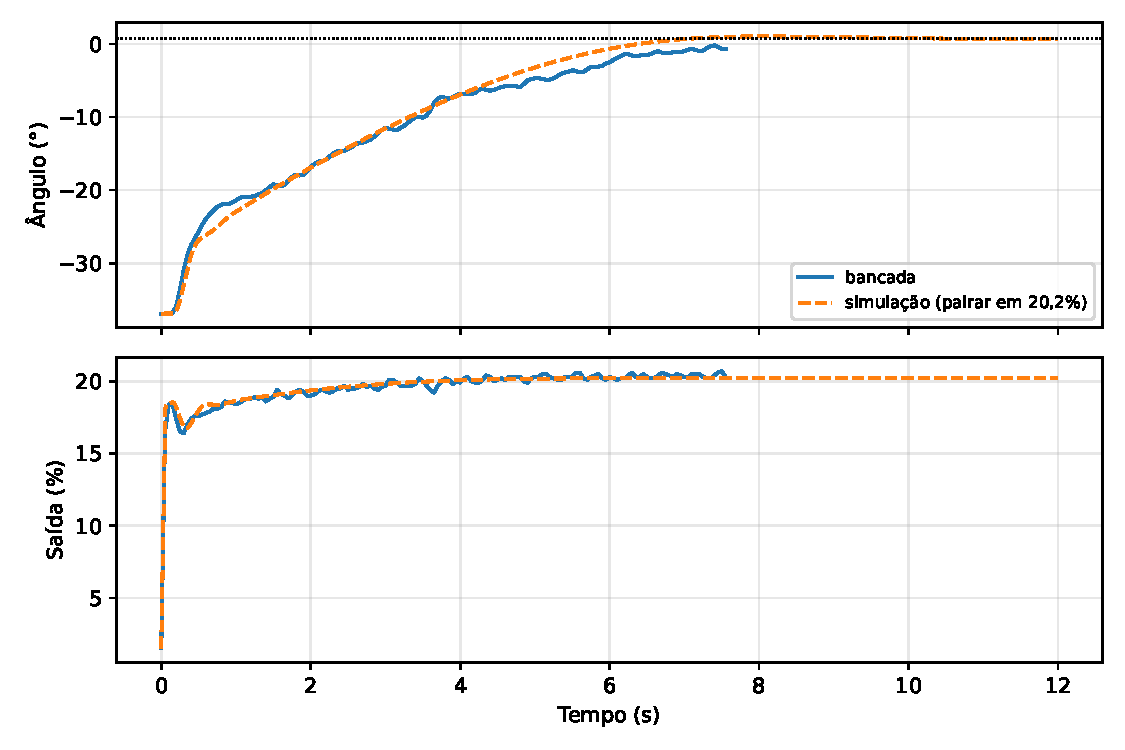
\includegraphics[width=.85\textwidth]{results/partida_real_vs_sim.pdf}
\fonte{Elaborado pelos autores (2026), dados da bancada e simulação com a planta identificada.}
\end{figure}
A simulação, ajustada ao PWM de pairar medido (20,2\%), previu 5,7~s para a mesma partida, ou seja, 14\% menos que o observado; a forma da curva e a saída final coincidem. Em 15,9~s de voo pairando, o ângulo ficou entre $-0{,}1^\circ$ e $1{,}6^\circ$, com média de $0{,}74^\circ$ e desvio padrão de $0{,}33^\circ$, e a saída ficou entre 19,9\% e 20,8\% (média de 20,3\%). A média coincide com o alvo, o que mostra que o controle segue a estimativa de ângulo; a posição física da haste perto da horizontal foi conferida visualmente, sem instrumento.

\section{FILTRO COMPLEMENTAR: COM E SEM FILTRO}

Esta coleta foi feita com a primeira versão do filtro, em que o ângulo em voo vinha só do giroscópio. O ângulo calculado só pelo acelerômetro (``sem filtro'') foi refeito a partir das acelerações X e Z registradas e comparado com o ângulo do firmware. Em repouso, no primeiro registro, os dois diferem em $0{,}2^\circ$ ($-37{,}1^\circ$ contra $-36{,}9^\circ$). Em voo pairando, o acelerômetro tem média de $6{,}4^\circ$, desvio padrão de $8{,}3^\circ$ e extremos de $-9{,}5^\circ$ a $+32{,}7^\circ$, contra desvio de $0{,}33^\circ$ e extremos de $-0{,}1^\circ$ a $1{,}6^\circ$ do ângulo do firmware; a diferença quadrática média entre os dois é de $10{,}0^\circ$ (Figura~\ref{fig:filtro_pairando}). Na partida, a diferença quadrática média em voo foi de $8{,}3^\circ$ (Figura~\ref{fig:filtro_partida}).
\begin{figure}[htbp]
\centering\caption{Ângulo sem filtro (acelerômetro) e do firmware, com a haste pairando.}\label{fig:filtro_pairando}
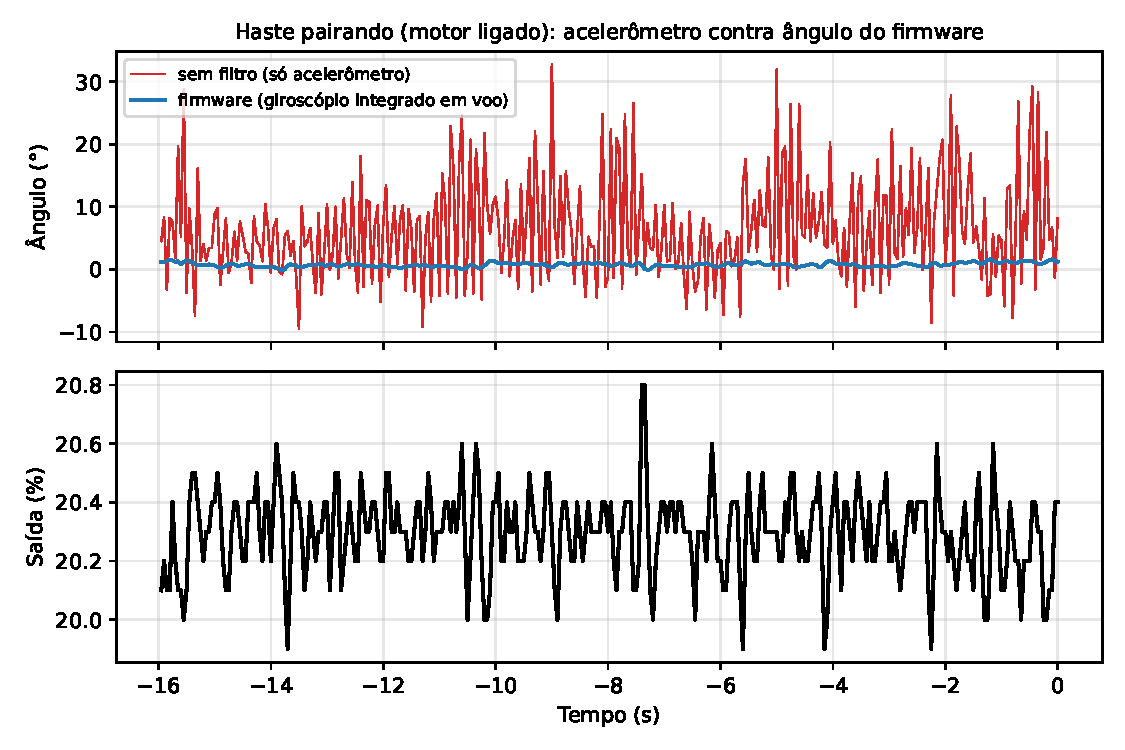
\includegraphics[width=.85\textwidth]{results/filtro_pairando.pdf}
\fonte{Elaborado pelos autores (2026), dados da bancada.}
\end{figure}
\begin{figure}[htbp]
\centering\caption{Ângulo sem filtro (acelerômetro) e do firmware na partida.}\label{fig:filtro_partida}
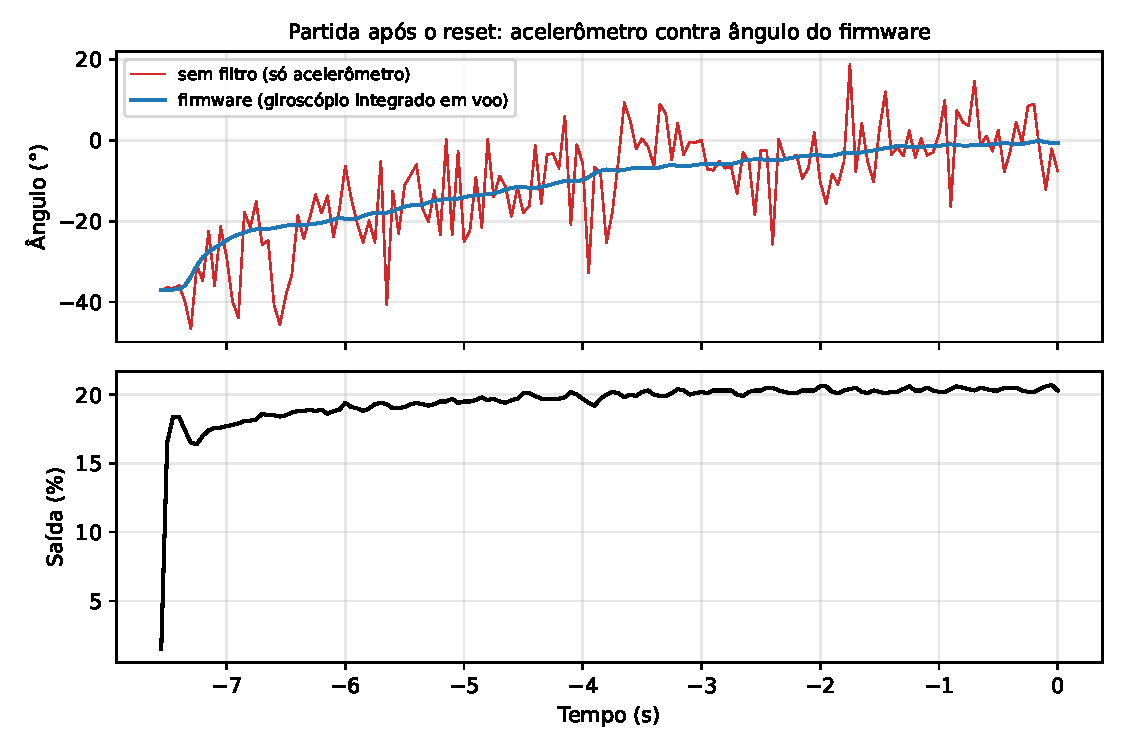
\includegraphics[width=.85\textwidth]{results/filtro_partida.pdf}
\fonte{Elaborado pelos autores (2026), dados da bancada.}
\end{figure}
Usar o acelerômetro direto no controle traria um erro de dezenas de graus e um desvio fixo de cerca de $+6^\circ$. Por isso ele nunca entra direto no controle: na versão final, só corrige o ângulo devagar (Seção~\ref{sec:deriva}). Uma limitação: em voo não há outra referência de ângulo para conferir o giroscópio. A comparação mostra que o acelerômetro não é confiável com a hélice girando, mas não mede o erro do ângulo do firmware. O ensaio de movimento manual com o motor desligado, que mostraria o acelerômetro e o giroscópio concordando, não foi registrado nesta coleta.

\section{PID COM E SEM ANTI-\textit{WINDUP}}

Na bancada, a saída máxima da partida foi de 20,7\%, abaixo do limite de 32\%, de modo que a integração condicional nunca foi acionada. Para conferir, o PID do firmware foi refeito sobre o ângulo e a velocidade medidos, com e sem a integração condicional: as duas saídas foram idênticas, e a saída refeita terminou em 20,4\%, contra 20,3\% da real. Isso valida a reprodução do PID no computador e mostra que, com os ganhos de projeto, o anti-\textit{windup} não altera o comportamento nesta partida. Seu efeito aparece quando a saída satura ou os ganhos são altos, como mostra a simulação (Tabela~\ref{tab:windup}). O firmware final tem uma chave de ensaio (\texttt{aw=0|1} pelo ST-Link), ligada por padrão, que desativa só a integração condicional e mantém o limite do integrador; a comparação na bancada com ela não foi realizada.

\section{DERIVA DO GIROSCÓPIO E CORREÇÃO EM VOO}

Com a primeira versão do filtro (em voo, só giroscópio), a haste segurada no zero físico foi lida pelo acelerômetro em $-1{,}9^\circ$ (média, mediana $-1{,}4^\circ$), enquanto o firmware marcava $+11{,}6^\circ$ após 204~s ligado: 13,5$^\circ$ de erro em 190~s, ou cerca de $4^\circ$/min (Seção~\ref{sec:deriva}). Depois de gravar a versão com correção lenta pelo acelerômetro em voo ($\tau=30$~s, janela de $25^\circ$), a mesma comparação, com a haste pairando sozinha, deu:
\begin{table}[htbp]
\centering\caption{Ângulo do firmware e do acelerômetro em voo, antes e depois da correção.}\label{tab:deriva}
\begin{tabularx}{\textwidth}{Xrrr}
\hline\textbf{Situação} & \textbf{Firmware} & \textbf{Acelerômetro (média)} & \textbf{Diferença}\\\hline
Sem correção, 204~s ligado (haste segurada no zero) & $11{,}6^\circ$ & $-1{,}9^\circ$ & $13{,}5^\circ$\\
Com correção, 130~s ligado (pairando) & $0{,}53^\circ$ & $1{,}4^\circ$ & $0{,}9^\circ$\\
Com correção, 174~s ligado (pairando) & $0{,}77^\circ$ & $2{,}8^\circ$ & $2{,}0^\circ$\\\hline
\end{tabularx}
\fonte{Elaborado pelos autores (2026), dados da bancada em 02/11/2026.}
\end{table}
Com a correção, a diferença caiu de 13,5$^\circ$ para 1 a 2$^\circ$, e o desvio do ângulo do firmware ficou em $0{,}37^\circ$ (extremos de $-0{,}1^\circ$ a $1{,}9^\circ$). A diferença restante é a polarização do acelerômetro em voo, de $+1{,}4^\circ$ a $+2{,}8^\circ$ nestas leituras. O zero físico não foi conferido em voo com um instrumento externo. A única referência externa é a medida feita com a haste parada e segurada no nível do celular, em que o acelerômetro marcou de $-1{,}4^\circ$ a $-1{,}9^\circ$. Assim, o zero físico pode diferir do zero do firmware em alguns graus.

\section{DISTÚRBIOS}

Depois de um empurrão para cima ou para baixo, a haste volta ao alvo, mas com uma leve dificuldade de reassentar exatamente no ângulo desejado. As curvas desses ensaios não foram registradas. As causas prováveis são o integrador, que leva cerca de 7~s para se refazer com $K_i$ pequeno (Seção~\ref{sec:antiwindup}), e a deriva do giroscópio em voo, que na versão inicial chegou a $4^\circ$/min e agora é corrigida lentamente pelo acelerômetro.

\section{ESTABILIDADE DA EXECUÇÃO}

Em 34\,870 ciclos de controle (174~s) da versão final, e em 153\,773 ciclos (768~s) da anterior, não houve nenhuma falha de leitura do MPU6050, nenhum erro da UART e nenhum reinício do I\textsuperscript{2}C; em outras partidas da placa houve um reinício do barramento, recuperado sozinho, sem falha de leitura. A folga mínima de pilha foi de 289, 139 e 127 palavras nas tarefas \texttt{control}, \texttt{cmd} e \texttt{telem} (Seção~\ref{sec:temporal}). O corte por ângulo não foi acionado nesta coleta.

\section{DESEMPENHO TEMPORAL}

Com o contador de ciclos do DWT (Seção~\ref{sec:temporal}), em 34\,870 ciclos (174~s) da versão final: atraso entre a interrupção do TIM2 e o PWM escrito de no máximo 579,5~$\mu$s (média de 557,6~$\mu$s, 99,82\% entre 550 e 600~$\mu$s), 11,6\% do prazo de 5~ms; nenhum tick perdido e nenhum ciclo acima de 5~ms; \textit{jitter} do intervalo entre interrupções de 11,2~$\mu$s no pior ciclo (4\,998,3 a 5\,009,5~$\mu$s); \textit{heap} com 4\,168~bytes livres (menor folga de 3\,472~bytes); Flash de 42~kB. Os valores medidos ficaram dentro das estimativas de projeto.

\chapter{MELHORIA E REFINO}\label{cap:refino}

Os ganhos do PID de projeto ($K_p=0{,}06$, $K_i=0{,}05$, $K_d=0{,}04$, com anti-\textit{windup} por integração condicional) tinham sido escolhidos pela margem de fase (Capítulo~\ref{cap:processo}) e pareciam o estado final. Com o firmware instrumentado e a chave de ensaio do anti-\textit{windup}, foi possível testar outros valores na própria bancada, sem regravar, e escolher com base em medições.

\section{PROCEDIMENTO}

Foram avaliados cinco conjuntos (Tabela~\ref{tab:refino_conj}), escolhidos por margem de fase de pior caso de pelo menos $30^\circ$ no modelo identificado (\texttt{firmware/tools/arm\_margins.py}). Para cada conjunto os ganhos foram escritos na RAM pelo ST-Link, a haste estabilizou por 20~s e foram registradas $N=1\,200$ amostras (60~s a 20~Hz) do ângulo estimado pelo MPU6050, da velocidade e da saída. Em seguida, com os mesmos ganhos, foram aplicados degraus de \textit{setpoint} de $+10^\circ$, $-20^\circ$ e volta ao alvo ($0{,}7^\circ$), com 12~s em cada patamar. O registro de 16~s da RAM é lido várias vezes e costurado pelo índice da amostra (\texttt{firmware/tools/captura\_longa.py} e \texttt{firmware/tools/captura\_degraus.py}); as 60 amostras mais antigas de cada leitura são descartadas porque a leitura não é atômica. Duas coletas de regime foram refeitas porque tiveram perturbações externas (desvios de mais de $3^\circ$ por poucos segundos).
\begin{table}[htbp]
\centering\caption{Conjuntos de ganhos testados.}\label{tab:refino_conj}
\begin{tabularx}{\textwidth}{llllX}
\hline\textbf{Teste} & $K_p$ & $K_i$ & $K_d$ & \textbf{Anti-\textit{windup}}\\\hline
T1 (projeto) & 0,06 & 0,05 & 0,04 & integração condicional\\
T2 & 0,06 & 0,05 & 0,04 & desligado (só limita o integrador)\\
T3 & 0,06 & 0,08 & 0,04 & integração condicional\\
T4 & 0,08 & 0,08 & 0,04 & integração condicional\\
T5 & 0,06 & 0,09 & 0,04 & integração condicional\\\hline
\end{tabularx}
\fonte{Elaborado pelos autores (2026).}
\end{table}

\section{RESULTADOS EM REGIME}

Com a haste pairando, os cinco conjuntos ficaram praticamente iguais (Tabela~\ref{tab:refino_regime}, Figura~\ref{fig:refino_paineis}): erro quadrático médio (RMS) de $0{,}29^\circ$ a $0{,}32^\circ$ e pico a pico de $1{,}7^\circ$ a $2{,}0^\circ$. O ângulo é registrado com resolução de $0{,}1^\circ$, e as diferenças entre testes ficam dentro do ruído. Em regime, portanto, os ganhos testados não se distinguem.
\begin{table}[htbp]
\centering\caption{Regime, $N=1\,200$ amostras (60~s) por teste.}\label{tab:refino_regime}
\begin{tabularx}{\textwidth}{Xrrrr}
\hline\textbf{Teste} & \textbf{Média ($^\circ$)} & \textbf{RMS do erro ($^\circ$)} & \textbf{Pico a pico ($^\circ$)} & \textbf{Máx. $|e|$ ($^\circ$)}\\\hline
T1 & 0,71 & 0,30 & 1,8 & 1,0\\
T2 & 0,60 & 0,31 & 1,8 & 1,1\\
T3 & 0,65 & 0,32 & 2,0 & 1,1\\
T4 & 0,59 & 0,30 & 1,7 & 0,9\\
T5 & 0,62 & 0,29 & 1,8 & 1,0\\\hline
\end{tabularx}
\fonte{Elaborado pelos autores (2026), dados da bancada em 02/11/2026. Erro em relação ao alvo de $0{,}7^\circ$.}
\end{table}
\begin{figure}[htbp]
\centering\caption{Ângulo estimado pelo MPU6050 nos cinco testes, em regime.}\label{fig:refino_paineis}
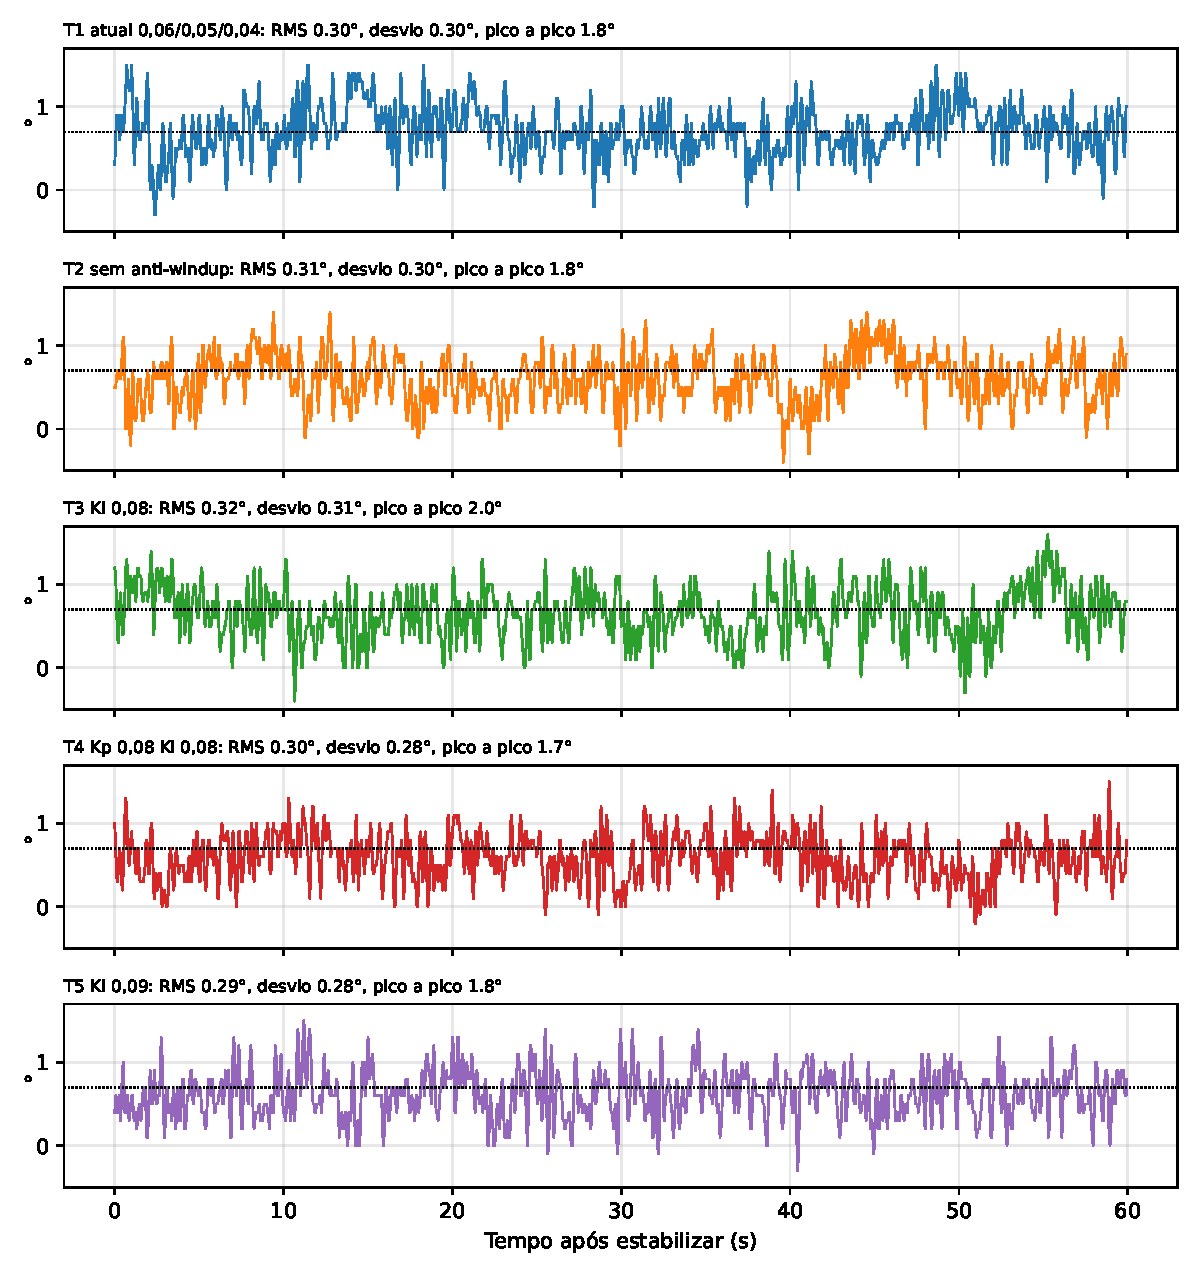
\includegraphics[width=.9\textwidth]{results/refino_paineis.pdf}
\fonte{Elaborado pelos autores (2026), dados da bancada.}
\end{figure}

\section{RESPOSTA A DEGRAUS}

Nos degraus, os conjuntos se separam (Tabela~\ref{tab:refino_degraus}, Figuras~\ref{fig:refino_degraus} e~\ref{fig:refino_degraus_metricas}). O erro acumulado (IAE, integral do módulo do erro, nas três janelas de 12~s) foi de 94,6$^\circ$\,s para o T3 contra 132,0$^\circ$\,s para o T1, 28\% menor. O $K_i$ maior acelera a volta: o tempo para chegar a 90\% do degrau de $-20^\circ$ caiu de 7,5~s (T1) para 4,0~s (T3), e o do retorno ao alvo, de 6,1~s para 3,3~s. O sobressinal do degrau de $+10^\circ$ ficou entre 26\% e 32\% em todos os conjuntos, e portanto não depende dos ganhos testados; reduzi-lo exigiria outra medida, como filtrar o \textit{setpoint}.
\begin{table}[htbp]
\centering\caption{Resposta a degraus de \textit{setpoint}.}\label{tab:refino_degraus}
\begin{tabularx}{\textwidth}{Xrrrrr}
\hline\textbf{Teste} & \textbf{IAE total ($^\circ$\,s)} & \textbf{$t_{90}$ de $+10^\circ$ (s)} & \textbf{$t_{90}$ de $-20^\circ$ (s)} & \textbf{$t_{90}$ da volta (s)} & \textbf{Sobressinal $+10^\circ$ (\%)}\\\hline
T1 & 132,0 & 2,35 & 7,50 & 6,05 & 31,6\\
T2 & 145,4 & 2,90 & 8,00 & 5,55 & 26,6\\
T3 & \textbf{94,6} & 1,95 & 4,00 & 3,25 & 27,2\\
T4 & 109,4 & 1,95 & 4,60 & 4,25 & 26,0\\
T5 & 111,0 & 1,45 & 4,15 & 3,65 & 32,2\\\hline
\end{tabularx}
\fonte{Elaborado pelos autores (2026), dados da bancada em 02/11/2026. Janela de 12~s por degrau.}
\end{table}
\begin{figure}[htbp]
\centering\caption{Resposta aos degraus de \textit{setpoint} nos cinco testes.}\label{fig:refino_degraus}
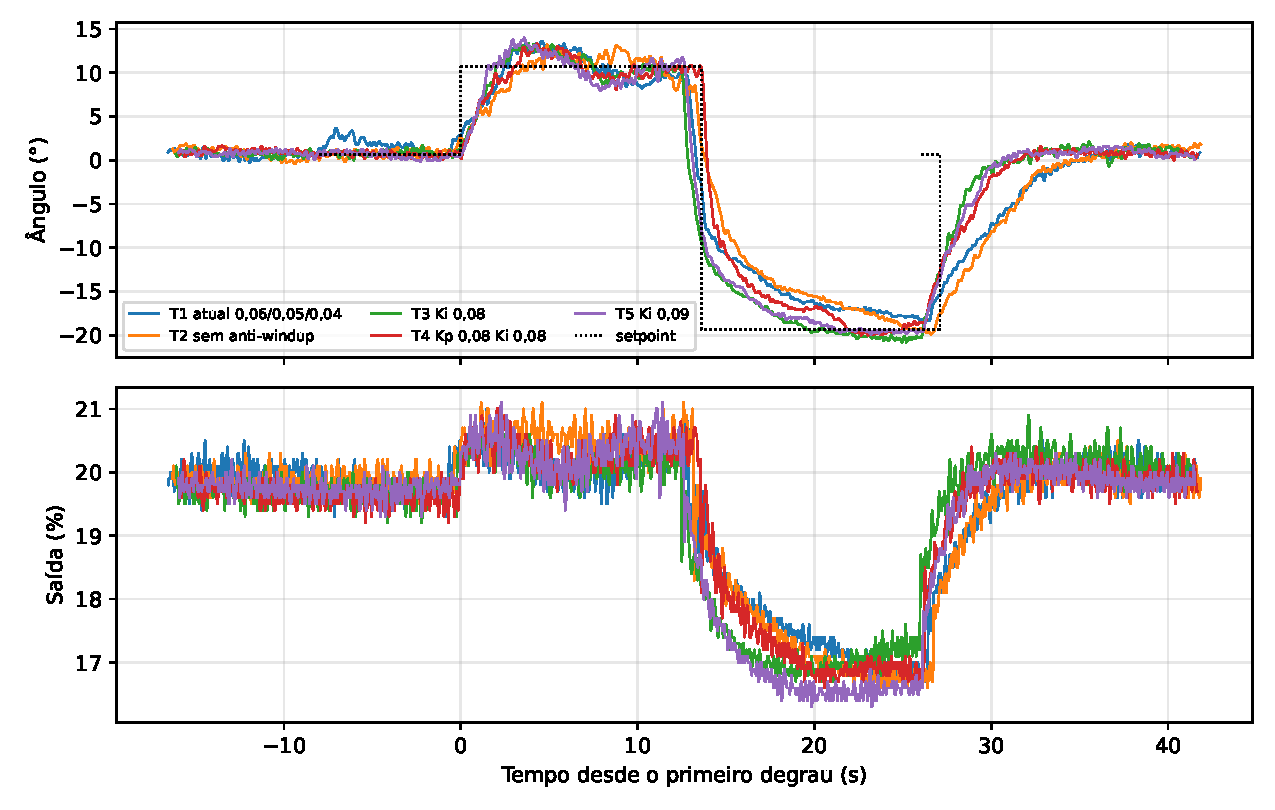
\includegraphics[width=.95\textwidth]{results/refino_degraus.pdf}
\fonte{Elaborado pelos autores (2026), dados da bancada.}
\end{figure}
\begin{figure}[htbp]
\centering\caption{Métricas dos degraus por teste.}\label{fig:refino_degraus_metricas}
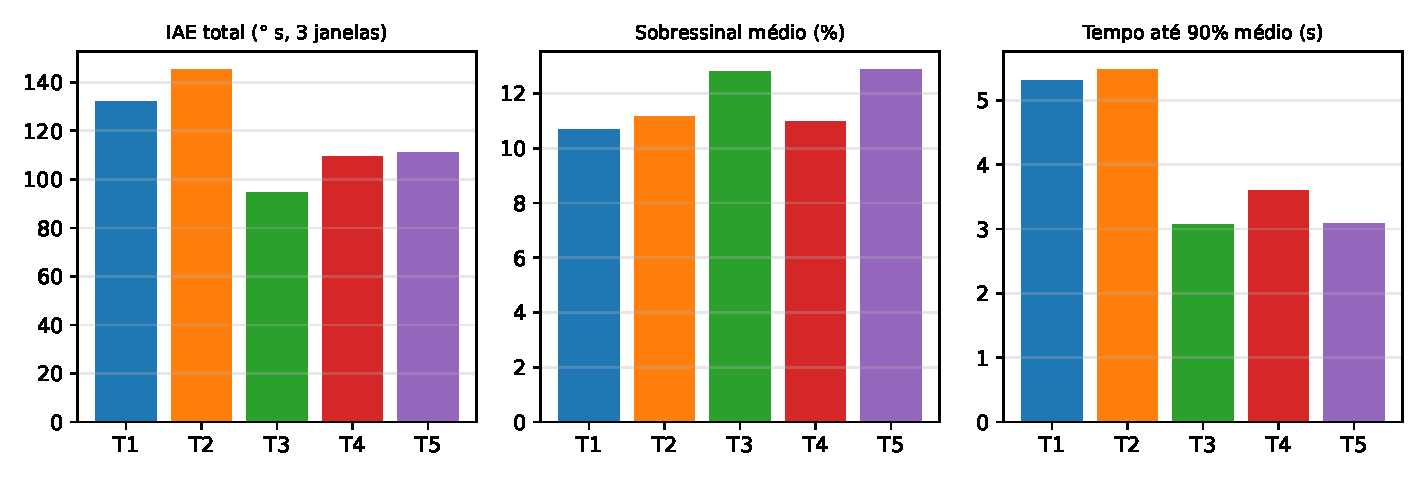
\includegraphics[width=.95\textwidth]{results/refino_degraus_metricas.pdf}
\fonte{Elaborado pelos autores (2026), dados da bancada.}
\end{figure}

\section{ANTI-\textit{WINDUP} NA BANCADA}

A comparação do T1 (com a integração condicional) com o T2 (sem ela) mostrou 9\% a mais de erro acumulado no T2, mas isso não pode ser atribuído ao \textit{windup}: nos degraus, a saída variou de 16,0\% a 21,1\%, sem tocar nos limites de 10\% e de 32\%, de modo que a integração condicional nunca foi acionada. A diferença está dentro da repetibilidade medida: o mesmo conjunto de ganhos do T3, repetido na validação final, deu IAE de 101,5$^\circ$\,s contra 94,6$^\circ$\,s, 7\% de diferença entre execuções. A bancada, nesta faixa de operação, não excita o \textit{windup}; a evidência de que ele importa vem da simulação com ganhos altos e saturação (Seção~\ref{sec:antiwindup}). O anti-\textit{windup} foi mantido ligado por ser uma proteção sem custo.

\section{DECISÃO E ESTADO FINAL}

Foi escolhido o conjunto T3 ($K_p=0{,}06$, $K_i=0{,}08$, $K_d=0{,}04$, com anti-\textit{windup}): menor erro acumulado nos degraus, mesma margem de fase de pior caso do projeto ($32{,}5^\circ$) e regime indistinguível dos demais. T4 e T5 ficaram de 15\% a 17\% acima, pouco mais que o dobro da repetibilidade, e T1 e T2 foram claramente piores. Como $K_i=0{,}08$ passou a ser o valor padrão em \texttt{app\_config.h}, o firmware foi regravado, e o conjunto foi validado de novo (Tabela~\ref{tab:refino_final}).
\begin{table}[htbp]
\centering\caption{Estado final: validação do firmware regravado com $K_i=0{,}08$.}\label{tab:refino_final}
\begin{tabularx}{\textwidth}{Xr}
\hline\textbf{Grandeza} & \textbf{Valor}\\\hline
Regime, $N=1\,200$: média / RMS do erro / pico a pico / máx. $|e|$ & $0{,}67^\circ$ / $0{,}28^\circ$ / $1{,}4^\circ$ / $0{,}7^\circ$\\
Degraus: IAE total & 101,5$^\circ$\,s\\
Degraus: $t_{90}$ de $+10^\circ$ / de $-20^\circ$ / da volta & 2,3~s / 4,25~s / 3,9~s\\
Ciclos, ticks perdidos, atrasos de prazo, cortes por ângulo & 34\,870, 0, 0, 0\\
Latência interrupção até PWM (máx. / média) & 579,5~$\mu$s / 557,6~$\mu$s\\\hline
\end{tabularx}
\fonte{Elaborado pelos autores (2026), dados da bancada em 02/11/2026.}
\end{table}
O estado final do trabalho é, portanto, o conjunto refinado, e não o dos ganhos de projeto: o desempenho em regime é o mesmo, mas o erro acumulado nos degraus é cerca de 28\% menor.

\clearpage
\chapter{CONSIDERAÇÕES FINAIS}
Este trabalho apresentou o projeto, a construção e a avaliação de uma haste de um grau de liberdade estabilizada por empuxo, empregada como estudo de caso para a aplicação do FreeRTOS a um sistema de controle crítico. As tarefas foram divididas segundo o período e a criticidade: a cadeia sensor, filtro, PID e motor roda em uma única tarefa, acordada a cada 5~ms por um semáforo liberado pelo TIM2, e comandos e telemetria ficam em tarefas de menor prioridade, que não conseguem atrasá-la. Medido no microcontrolador, o atraso entre a interrupção e o PWM foi de no máximo 580~$\mu$s, 11,6\% do período, sem nenhum ciclo perdido. Os módulos, a configuração do STM32 e as versões das ferramentas estão documentados para permitir a replicação.

Parte significativa do aprendizado decorreu dos problemas enfrentados na bancada. O aquecimento do motor foi atribuído à corrente pulsada do PWM sobre um motor de indutância muito baixa e resolvido com um indutor em série. Com a hélice em rotação, o acelerômetro deixou de ser confiável, e o ângulo em voo passou a ser obtido apenas pelo giroscópio; o viés deste, contudo, provocou uma deriva de cerca de $4^\circ$/min e, na ausência de corte por ângulo, a haste chegou a completar uma volta. A solução foi o corte por ângulo e uma correção muito lenta pelo acelerômetro em voo, que reduziu a diferença entre o ângulo do firmware e o do acelerômetro de 13,8$^\circ$ para 1 a 2$^\circ$. O ajuste do PID mostrou que, com atraso de empuxo de dezenas de milissegundos, ganhos altos oscilam e que a integração condicional evita o \textit{windup}; a simulação com a planta identificada quantificou esse efeito.

O refino na bancada, com cinco conjuntos de ganhos, 1\,200 amostras em regime e degraus de \textit{setpoint} em cada um, mostrou que em regime todos são equivalentes (erro quadrático médio de $0{,}29^\circ$ a $0{,}32^\circ$) e que nos degraus $K_i=0{,}08$ reduz o erro acumulado em 28\% em relação aos ganhos de projeto; esse foi o estado final adotado e regravado. A bancada, entretanto, não leva a saída à saturação e, por isso, não exercita o anti-\textit{windup}, cujo efeito foi evidenciado apenas na simulação com ganhos elevados.

Como limitações do trabalho, destacam-se: a medição de tempo foi feita com a telemetria ativa e não prova o pior caso; as curvas de distúrbio e o ensaio do acelerômetro com o motor desligado não foram registrados; o ângulo em voo depende de uma correção lenta pelo acelerômetro, com erro fixo igual à polarização dele, ainda não conferida com um nível externo; não há \textit{watchdog} independente, de modo que uma falha do processador deixa o PWM no último valor. Como trabalhos futuros, sugerem-se: repetir a medição de tempo sem a telemetria, adicionar um \textit{watchdog} e a verificação de estouro de pilha, conferir o zero físico com um nível externo, ler o sensor por DMA e disparar o ciclo pelo pino de dado pronto do MPU6050.

\clearpage

\makeatletter
\renewcommand{\bibsection}{%
    \cleardoublepage
    \phantomsection
    \Hy@raisedlink{\hyper@anchorstart{referencias.titulo}\hyper@anchorend}%
    \def\@currentHref{referencias.titulo}%
    \addcontentsline{toc}{chapter}{REFERÊNCIAS}
    \begin{flushleft}
        \chaptitlefont\MakeTextUppercase{\bibname}
    \end{flushleft}
    \vspace{\afterchapskip}
}
\makeatother
\begin{SingleSpace}
\RaggedRight
\interlinepenalty=10000
\setlength{\bibitemsep}{2\baselineskip}
\bibliography{references}       
\end{SingleSpace}

\end{document}
